\documentclass[a4paper, 11pt]{article}
\usepackage[utf8]{inputenc}
\usepackage[T1]{fontenc}
\usepackage[english]{babel}
\usepackage{amsmath, amssymb, amsthm}
\usepackage{geometry}
\usepackage{enumitem}
\usepackage{hyperref}
\usepackage{dirtytalk}
\usepackage{listings}
\usepackage{array}
\usepackage{tcolorbox}
\usepackage{tikz}
\usepackage{pifont} 
\usepackage{rotating}
\usepackage[acronym]{glossaries}
\usepackage[utf8]{inputenc}
\usepackage{pgffor}
\usepackage[font=small,labelfont=bf]{caption} % Required for specifying captions to tables and figures
\newacronym{os}{OS}{Operating System}

\newcommand{\cmark}{\ding{51}} 
\newcommand{\xmark}{\ding{55}}
\usetikzlibrary{decorations.pathreplacing}
\usetikzlibrary{matrix, arrows.meta, positioning}
\geometry{left=2.5cm, right=2.5cm, top=2.5cm, bottom=2.5cm}
\newcommand{\allocStorageStruct}[2]{
	\draw (#1, #2) rectangle (#1+6, #2+6);
	\draw (#1, #2+5) -- (#1+6, #2+5);
	\node at (#1+3, #2+5.5) {Next};
	\node at (#1+3, #2+2.5) {Byte array};
}
\newcommand{\listnode}[3]{
			\allocStorageStruct{#1}{#2}
			\draw[->] (#1+6, #2+5.5) -- (#1+7, #2+5.5);
			\ifnum#3=1
				\node at (#1+8, #2+5.5) {NULL};
			\fi
}

\newcommand{\ptraddress}[1]{%
    0x\textcolor{gray}{\scalebox{0.9}{fffffff}}#1%
}


\makenoidxglossaries  


\newacronym{cheri}{CHERI}{Capability Hardware Enhanced RISC Instructions}
\newacronym{darpa}{DARPA}{Defense Advanced Research Projects Agency }
\newacronym{ssith}{SSITH}{System Security Integration Through Hardware and Firmware }
\newacronym{isa}{ISA}{Instructions Set Architecture}
\newacronym{risc}{RISC}{Reduced Instruction Set Computer}
\newacronym{llvm}{LLVM}{Low Level Virtual Machine}
\newacronym{cisc}{CISC}{Complex Instruction Set Computer}
\newacronym{rtos}{RTOS}{Real Time Operating System}
\newacronym{qemu}{QEMU}{Quick Emulator}
\newacronym{dos}{DOS}{Denial Of Service}
\newacronym{gdb}{GDB}{GNU Debugger}
\newacronym{mpu}{MPU}{Memory Protection Unit}
\newacronym{ecu}{ECU}{Electronic Control Unit}
\newacronym{mmu}{MMU}{Memory Management Unit}
\newacronym{ffi}{FFI}{Foreign Function Interface}
\newacronym{ddl}{DDL}{Dynamic Link Library}
\newacronym{dram}{DRAM}{Dynamic Random Access Memory}
\newacronym{abi}{ABI}{Application Binary Interface}
\newacronym{fpga}{FPGA}{Field programable Gate Array}
\newacronym{rop}{ROP}{Returned Oriented programing}
\newacronym{ipc}{IPC}{Inter Process Communication}

\newglossaryentry{risc-v}
{
        name=RISC-V,
        description={open standard instruction set architecture (ISA) based on established reduced instruction set computer (RISC) principles}
}

\newglossaryentry{cheri-risc-v}
{
        name=CHERI-RISC-V,
        description={Implementation of CHERI hardware protection on RISC-V architecture}
}

\newglossaryentry{freertos}
{
        name=FreeRTOS,
        description={open source real time operating system}
}

\newglossaryentry{cheribsd}
{
        name=CheriBSD,
        description={Capability enabled Unix-like Operating System, using CHERI-RISC-V architecture, forking FreeBSD}
}

\newglossaryentry{morello}
{
        name=ARM Morello,
        description={Capability enabled Unix like Operating System, using Armv8-A architecture}
}
\newglossaryentry{cheri-freertos}
{
        name=CHERI-FreeRTOS,
        description={Capability enabled real time operating system, fork of Freertos, using CHERI-RISC-V architecture}
}
\newglossaryentry{baremetal}
{
        name=baremetal,
        description={program used directly on the hardware, without an interface such as an operating system}
}
\newglossaryentry{cross-compilation}
{
        name=cross-compilation,
        description={compilation executed from a certain architecture to another one (e.g. CISC to RISC)}
}
\newglossaryentry{race-condition}
{
        name=race-condition,
        description={A race condition or race hazard is the condition of an electronics, software, or other system where the system's substantive behavior is dependent on the sequence or timing of other uncontrollable events, leading to unexpected or inconsistent results. It becomes a bug when one or more of the possible behaviors is undesirable.}
}


 %\gls{risc-v} \Glspl{cisc}
%\Gls{cheribsd}
 %\acrlong{llvm} \acrshort{llvm} \acrfull{ssith}.


\title{CHERI Exercises, Solutions and Explanations}
\author{Le Botlan Pierre-Gilles \\\textit{Research Project Student} \\ \textit{Cybersecurity Research Group} \\ \textit{Nottingham Trent University} }

\definecolor{lightblue}{RGB}{173, 216, 230}
\definecolor{darkgreen}{rgb}{0.0, 0.5, 0.0}

\lstset{ %
  language=C,                   % Code language
  backgroundcolor=\color{gray!20}, % set background color
  basicstyle=\footnotesize\ttfamily, % set font style
  breaklines=true,              % automatic line breaking
  captionpos=b,                 % sets the caption-position to bottom
  keywordstyle=\color{red},    % keyword style
  commentstyle=\color{gray},    % comment style
  stringstyle=\color{darkgreen},      % string literal style
  frame=lines                   % add a frame around the code
  showspaces=false,             % do not show spaces
  showstringspaces=false,        % do not show spaces in strings
  fontadjust=true,              % adjust font to reduce character spacing
  columns=fullflexible         % make columns flexible to reduce spacing
  }

  \hypersetup{
    colorlinks=true,
    linkcolor=blue,
    filecolor=magenta,      
    urlcolor=cyan,
}

\begin{document}

\maketitle
\tableofcontents
\addcontentsline{toc}{section}{Content Table}

\section{Introduction}
In this document, you will find condensed information about \Gls{cheri} to give a basic context of the hardware protection, some complementary explanations of the solutions from the \href{https://ctsrd-cheri.github.io/cheri-exercises/cover/index.html}{Adversarial CHERI Exercises and Missions} as well as some explanations of self-made tests inspired by CHERI Introduction to C/C++ \cite{watson2020cheri}, and finally some explanations concerning the Cyberphys demonstration. 
If you want to run these exercises yourself, you will need to follow the steps of this \href{https://ctsrd-cheri.github.io/cheri-faq/#how-can-i-emulate-a-cheri-enabled-environment}{official CHERI tutorial} on how to get CHERI environment. This will help you emulate using \Gls{qemu} either a \Gls{cheribsd} running on \Gls{cheri-risc-v} or \Gls{morello} environment. Take the \Gls{morello} environment to install useful packages such as llvm, gdb, python, nano, vim and many others.
These exercises will compare the behavior of CHERI protected environment and classic environment (\Gls{risc-v}). These CHERI exercises requires minimal knowledge of CHERI. The following section give essential information on the topic.
Note: This is not a research paper and does not have the vocation to be published. It is an explanation document.

\printnoidxglossaries


\section{CHERI Context}
Most of the following is a summary of the introduction to CHERI \cite{watson2019introduction}.
CHERI is an extension of the RISC instruction set (Reduces Instruction Set Computer)
This is the set of assembly instructions interpreted by a RISC-type processor (Reduced Instruction Set Computer), which constitute the elementary operations with which a program acts.
The aim of this extension is to prevent pointers from accessing memory areas that they should not be allowed to access. This is based on a hardware system of capabilities, hence CHERI relies on hardware protection.

The rights are partially present directly in the pointers themselves, as well as in a restricted-access memory zone. A CHERI pointer also includes bounds, rights and an object type. 
The restricted memory area contains a single bit associated with this pointer, corresponding to a validity tag.
Consequently the size of the pointer is now 128bits for 64-bit architecture (pointers now occupy 16 bytes instead of 8) and 64 bits for 32-bit architecture (CHERI was also designed to run on this older architecture for practical and compatibility reasons). 
All the pointers in a program are modified: explicit pointers (those declared directly by the programer, used to identify functions and variables) and implicit pointers (those silently introduced by compiler).

As a consequence, the compiler itself must be CHERI aware. For the time being, the CHERI project has adapted the C and C++ languages and has therefore developed its own version of the \acrshort{llvm} (Low Level Virtual Machine) compiler for these languages.
The modification in the nature of a pointer explain the modification of the instruction set: normal processor instructions will lead to errors or to an undesired sequence of operations, because they are not able to manipulate CHERI pointers as they are intended. 
\\\\
A CHERI pointer (also called a capability) is:
\begin{description}
	\item[An address] is what a normal pointer is: a reference to a place in memory.
	\item[A validity tag], a single bit located not in the pointer but in a safe zone in memory. It is a value which indicates whether a pointer can be dereferenced (read or modified). An invalid pointer can only be used to display its address. The values and rights of pointers can be modified under certain conditions. If a pointer modification is illegitimate, the validity tag is set to zero. (Following an unauthorized modification, it is considered that the pointer can no longer be trusted). 
	\item[Bounds] of a pointer define the lower and upper bounds which delimit the address range which a pointer can access. If a pointer attempts to access a memory area outside these bounds, a security exception is thrown.
	\item[Rights] of a pointer to a memory area are those of read, write value and capabilities (pointers) contained in that memory location. It depends on the architectural implementation but some common rights are execution, system calls and seal or unseal the capability.
	\item[An object type] is used to indicate the size of the object pointed to. If this value is set to -1, the pointer is no longer valid. It can be used by the compiler to fix bounds.
 \end{description}
\begin{figure}
	\begin{center}
	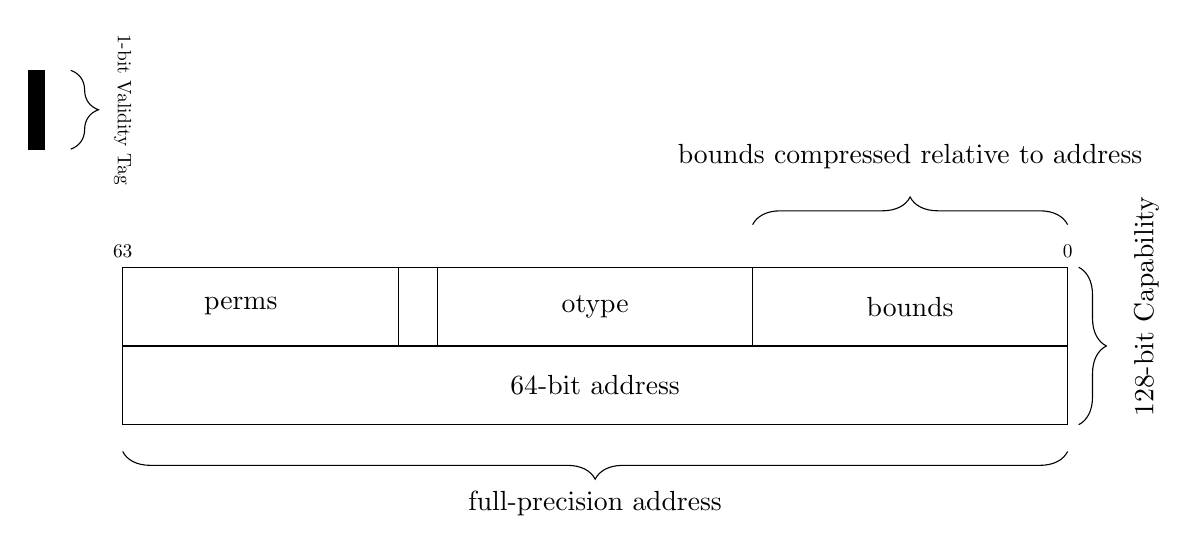
\begin{tikzpicture}
		% Draw the main rectangle for the full-precision address
		\draw (0,0) rectangle (12,2);
		
		% Draw the inner divisions for the capability
		\draw (0,1) rectangle (12,1);
		\draw (0,1) rectangle (3.5,2);
		\draw (3.5,1) rectangle (4,2);
		\draw (4,1) rectangle (8,2);
		\draw (8,1) rectangle (12,2);
		
		% Add labels for the sections
		\node at (1.5,1.5) {perms};
		\node at (6,1.5) {otype};
		\node at (10,1.5) {bounds};
		\node at (6,0.5) {64-bit address};
		
		% Add main label
		\node at (6, -1) {full-precision address};
		\node[rotate=-90, scale=0.7] at (0,4) {1-bit Validity Tag};
		\draw [decorate,decoration={brace,amplitude=10pt,mirror,raise=4pt}] (-0.8,3.5) -- (-0.8,4.5);
		\draw[fill=black] (-1.2,3.5) rectangle (-1,4.5);

		% Add the outer label for capability
		\draw [decorate,decoration={brace,amplitude=10pt,mirror,raise=4pt}] (12,0) -- (12,2) ;
		\node[rotate=90] at (13,1.5) {128-bit Capability};
		\draw [decorate,decoration={brace,amplitude=10pt,mirror,raise=4pt}] (0,-0.2) -- (12,-0.2) ;

		% Add the outer label for bounds compressed relative to address
		\draw [decorate,decoration={brace,amplitude=10pt,mirror,raise=4pt}]
			(12,2.4) -- (8,2.4) node [black,midway,yshift=1cm] {bounds compressed relative to address};
		
		% Add bit label
		\node[scale=0.7] at (0,2.2) {63};
		\node[scale=0.7] at (12,2.2) {0};

	\end{tikzpicture}
\end{center}
\caption{CHERI Pointers from An Introduction to CHERI paper}
\label{fig:ptr}
\end{figure}

 It is possible to display a pointer with more information about a CHERI system. For example, the following value is a pointer: 0x225300 [rwRW,0x225300-0x225301]. The address pointed to is: 0x225300. 
 The bounds are from 0x225300 to 0x225301. The upper bound is not included. It is therefore a pointer to a single byte, in this case a char.

CHERI protection focuses on three areas: {\bf Spatial safety}, {\bf Temporal safety} and {\bf Referential safety}.


\begin{description}
	\item[Spatial safety] guarantees that a pointer cannot under any circumstances read or write a memory area outside its bounds. It is important to note that bounds are compressed in their implementation in CHERI, so the precision is not exact. 
	This can be seen by assuming that bounds occupy 41 bits on a 64-bit architecture in cases requiring high precision.
	With 41 bits, we have an address space of $2^{41}$ values, whereas an address is written on 64 bits, i.e. having $2^{64}$ accessible values. However, memory allocations cannot accidentally overlap.
	\item[Temporal safety] prevents a pointer from accessing a memory area if it has been freed and then reallocated. On the other hand, a pointer can still access without error a deallocated memory that has not been reallocated.
	\item[Referential safety] aims to protect the pointers themselves, and includes two properties: integrity and original validity. Integrity ensures that corrupted pointers cannot be dereferenced, while original validity guarantees that a pointer derived (using pointer arithmetic) from an invalid pointer will also be invalid, and that a pointer from a valid pointer will be valid. Thus, only legitimate pointers and the pointers derived from them can be dereferenced.
\end{description}
Note that CHERI does not implement address randomization. Hence, pointers are likely to be identical from one execution to the other.\\
CHERI rights may be encoded differently depending on hardware implementation. For instance the localization of a bit corresponding to an access right may be different from one architecture to the other, making difficult to interpret a raw value for a right. For example with ARM-Morello, the bits refers to the capabilities of storing and loading data, execution, loading and storing capabilities (pointers), and other rights. 

In a study carried out by Microsoft in 2020 \cite{joly2020security}, a group of researchers studied which vulnerabilities were affected by CHERI protection. (see graphics \nameref{sec:tab} \nameref{sec:graph})
\begin{figure}[h!]
	
	\includegraphics[scale=0.5]{images/cheriMitigationTab.png}
	\caption{CHERI protection tab (Microsoft study)\cite{joly2020security}}
	\label{sec:tab}
\end{figure}
\begin{figure}[h!]
	
	\includegraphics[scale=0.4]{images/mitigationCHERIGraph.png}
	\caption{CHERI protection graph (Microsoft study)\cite{joly2020security}}
	\label{sec:graph}
\end{figure}
CHERI therefore offers complete protection against write and read accesses outside the limits imposed (spatial security property), possible protection against the use of freed memory (temporal safety of pointer to freed memory zone) and CHERI offers no protection against integer overflows (when an integer is incremented until it reaches the maximum value calculable with 4 bytes, it is reset to 0). 
\\
The study is no longer completely up-to-date, as CHERI now offers experimental protection against problems caused by memories that are not initialized correctly. It is possible to include options during compilation to force an initialization to 0 of all uninitialized bytes (NULL for a pointer).
In addition, temporal protections have been integrated into CHERI, as described in the article Cornucopia: Temporal Safety for CHERI Heaps \cite{filardo2020cornucopia}, which forbids the memory allocator to allocate a memory zone which is still pointed by a valid pointer (using a shadow bitmap, where one bit correspond to a word in memory, being the boolean: have this word been allocated and freed), and allows pointers to free zones to be "sweep" from memory using a specific operation, allowing re-use of those zone (setting the bit in the bitmap corresponding to that zone to 0). It does not prevent use after free until sweeping, however. Cornucopia also uses techniques to optimize memory scan, such as setting two flags for each memory pages: one standing for the absence of a pointer in the page, and one for the absence of pointer store since the last sweep (has a pointer been added to that page).
\\
According to a report on the compartmentalization provided by CHERI \cite{almatary2022compartos}, it is possible to use CHERI to implement strong compartmentalization in an embedded system, so that if an attacker were to exploit a vulnerability, the ability to interfere with the normal behavior of the system that he would obtain would be reduced compared with a conventional system. Indeed, even assuming the entirety of a non-critical compartment to be under the control of an attacker, the study demonstrates the normal operation of an embedded system using \Gls{cheri-freertos}, a \Gls{freertos} system using CHERI protections and CompartOS (the compartmentalization system dealt with in the study). On a standard \Gls{freertos} system running on \Gls{risc-v} architecture, the exploitation of a vulnerability is successful and the attacker can influence the integrity, confidentiality and availability of the data and the operation of the system. With CHERI protections under \Gls{cheri-freertos} running on \Gls{cheri-risc-v}, the attack is intercepted but the raising of an untreated error forces a brutal restart of the system, which takes two seconds, affecting the availability of the system playing a critical role (in the study, the system under attack was the brake system), with the use of CompartOS, the critical compartment is restarted in 60 microseconds and the malicious compartment is "killed". This study show different usage of compartmentalization, one enforced automatically using library linkage, another adding a custom handler which require knowledge of the compartmentalization process and implementation efforts but is necessary when dealing with a critical compartment (the study uses fault handling in different context: the main application, a non critical compartment and a critical compartment which is used by the main application).
A study carried out on Spectre-type attacks \cite{fuchs2021developing} showed that CHERI did not provide any protection against these attacks. Spectre-type attacks use an optimization flaw in the processors, which is not directly CHERI's area of intervention but are still considered memory vulnerabilities exploitation.
\clearpage
\section{CHERI Exercises}
\subsection{Demonstrate CHERI Tag Protection}
	This exercise demonstrate the validity tag protection utility.
	When modifying a pointer in a unauthorized way, it becomes invalid by setting automatically its validity tag to 0. Safe pointers have a validity tag of 1.
	It can be interpreted as a boolean for the capacity of the pointer to be dereferenced.
	Using the following we can define how to print a pointer (using standard print or verbose CHERI pointers specific print).
	\lstinputlisting[numbers=none, firstline=9, lastline=17, caption=]{code/ex1-corrupt-pointer.c}
	\%p print a standard pointer, while \%\#p prints CHERI information about the pointer.
	The objective here is to manipulate a pointer value in both authorized and not authorized ways and compare the behavior.
	\textbf{Take a moment to read the following code and comments}
	\lstinputlisting[numbers=none, firstline=21, lastline=28, caption=]{code/ex1-corrupt-pointer.c}
	The union is used in order to make possible byte modification (a pointer is 8 bytes in normal environment and 16 bytes on CHERI)
	Manipulating a pointer will manipulate all the bytes at the same time. Using byte array we can access specific parts of the pointer, and modify their value.
	\lstinputlisting[numbers=none, firstline=30, caption=]{code/ex1-corrupt-pointer.c}

To find the code, look for the github repository of the \href{https://github.com/CTSRD-CHERI/cheri-exercises}{CTSRD-CHERI/cheri-exercises} repository in the following path: src/exercises/cheri-tags/ . 


\begin{tcolorbox}[colback=gray!5!white, colframe=gray!75!black, title=Output on a classic \Gls{risc-v} environment (no CHERI Protection)]
buf=0x80a1ca60 \&p=0x80a1ca58\\
p.ptr=0x80a1cb6f (0x10f into buf) *p.ptr=0f\\
q=0x80a1cb00 (0xa0 into buf)\\
*q=a0\\
r=0x80a1cb00 (0xa0 into buf)\\
*r=a0
\end{tcolorbox}
In a classic environment execution, we see that all operations are allowed: the pointers obtained after the AND and the byte overwrite can both be dereferenced and their values printed.
If you are confused by the fact that the value pointed is 0xa0 into buf and not 0x100 into buf, remember that the mask and the modification to 0 on the last byte operations are on the address of p, not the index.
The two operation put the last byte on 0: 0x80a1cb6f  becomes 0x80a1cb00.

\begin{tcolorbox}[colback=gray!5!white, colframe=blue!75!black, title=Output on an environment protected by CHERI]
buf=\ptraddress{}7fd4c [rwRW, \ptraddress{}7fd4c-\ptraddress{}7ff4b]\\
\&p=\ptraddress{}7fd30 [rwRW,\ptraddress{}7fd30-\ptraddress{}7fd40]\\
p.ptr=\ptraddress{}7fe5b [rwRW,\ptraddress{}7fd4c-\ptraddress{}7ff4b]\\
 (0x10f into buf) *p.ptr=0f\\
q=\ptraddress{}7fe00 [rwRW, \ptraddress{}7fd4c-\ptraddress{}7ff4b] (0xb4 into buf)\\
*q=b4\\
r=\ptraddress{}7fe00 [rwRW, \ptraddress{}7fd4c-\ptraddress{}7ff4b] (invalid) (0xb4)\\
Program received signal SIGPROT, CHERI protection violation.\\
Capability tag fault
\end{tcolorbox}
The Capability Tag Fault is a security exception thrown because of a memory access through an invalid pointer. If you do the exercise, you will have "In-address space security exception (core dumped)" to obtain with more precision what kind of security error it is, its possible to use \Gls{gdb} to print with more information, in this case Capability tag fault. Capability Tag fault and Out of Bounds access are the most two frequent errors, but there is also an exception regarding rights. 
\begin{center}

	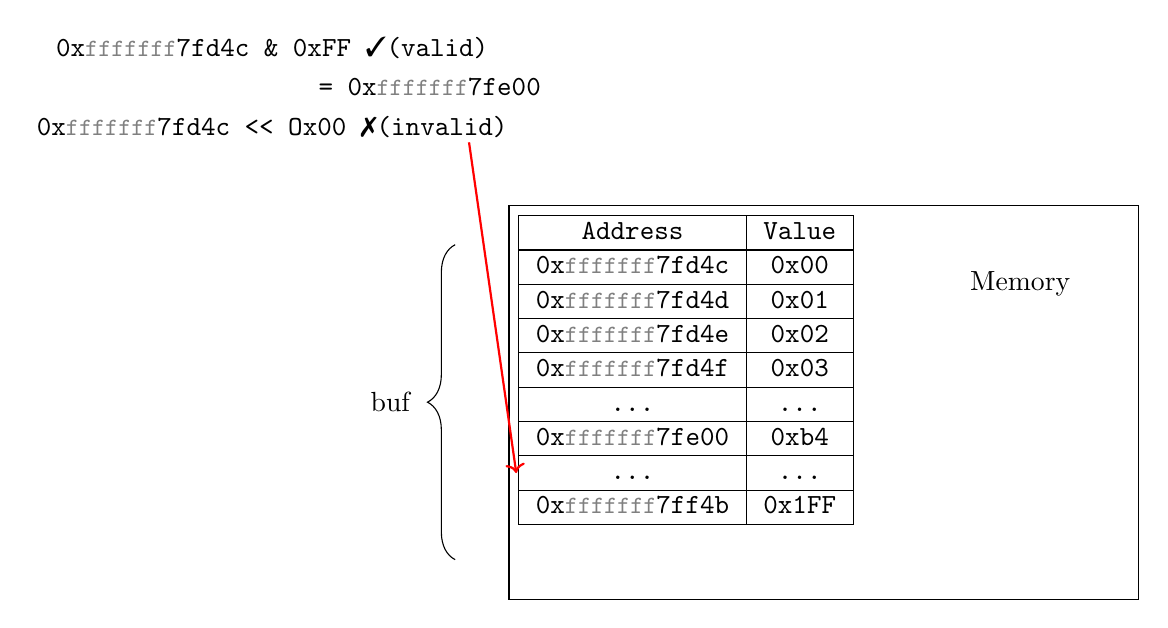
\begin{tikzpicture}
        \def\rows{5} 
        \def\cols{3}

        \node[draw, minimum width=8cm, minimum height=5cm, anchor=north west] (memory) at (0,0) {};

        \node[anchor=north west, font=\ttfamily] at (memory.north west) {
            \begin{tabular}{|c|c|}
                \hline
                \textbf{Address} & \textbf{Value} \\ \hline
                \ptraddress{}7fd4c & 0x00 \\ \hline
                \ptraddress{}7fd4d & 0x01 \\ \hline
                \ptraddress{}7fd4e & 0x02 \\ \hline
                \ptraddress{}7fd4f & 0x03 \\ \hline
                ... & ... \\ \hline
				\ptraddress{}7fe00 & 0xb4 \\ \hline
                ... & ... \\ \hline
                \ptraddress{}7ff4b & 0x1FF \\ \hline
            \end{tabular}
        };
		\node at (6.5, -1) {Memory};
		\draw [decorate,decoration={brace,amplitude=10pt,raise=5pt}] (-0.5, -4.5) -- (-0.5, -0.5) node [black,midway,xshift=-1cm] {buf};

        \draw[->, thick, red] (-0.5, 0.8) -- (0.1, -3.4);
        
        \node[font=\ttfamily] (pointer) at (-1, 1.5) {= \ptraddress{}7fe00};
		\node[font=\ttfamily] (pointer) at (-3, 2) {\ptraddress{}7fd4c \& 0xFF \cmark (valid)};
		\node[font=\ttfamily] (pointer) at (-3, 1) {\ptraddress{}7fd4c << Ox00 \xmark (invalid)};

    \end{tikzpicture}
	\end{center}
We can see here that the resulting pointer of the AND mask operation was considered valid whereas the pointer resulting of the byte modification was not considered valid. That is because a AND operation can verify if the resulting pointer is still in the bounds of the original pointer, if that is the case, its still valid, but if not it becomes invalid. Using a byte modification is not a valid modification of a pointer because its not supposed to happen. 
Invalid pointers can be printed, and they appear as invalid, hence can not be dereferenced. If trying to dereference them, as occurred during the execution, it produce the above error: SIGPROT, capability tag fault.

\subsection{Exercise an inter-stack-object buffer overflow}
	The objective of this exercise is to do a buffer overflow on the stack with two buffer next to each other, so that there's an overflow in an allocated memory.
	\textbf{Take a moment to read the following code and comments}
	\lstinputlisting[numbers=none, firstline=19, lastline=40, caption=]{code/ex2-buffer-overflow-stack.c}

	\begin{center}
		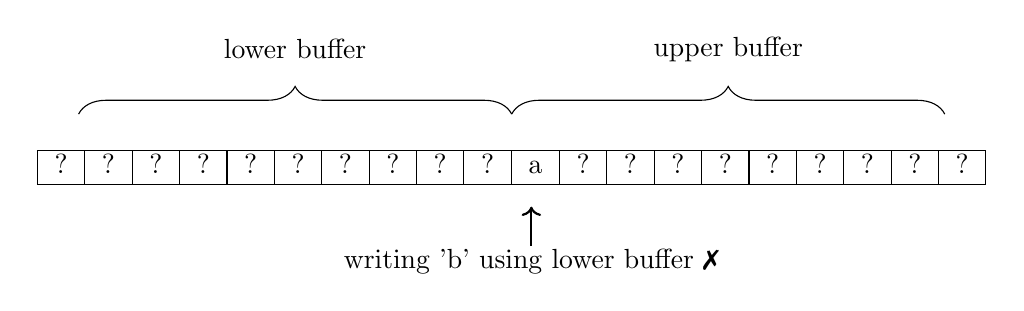
\begin{tikzpicture}
			\node (array) at (0, 0) {
				\begin{tabular}{|c|c|c|c|c|c|c|c|c|c|c|c|c|c|c|c|c|c|c|c|}
					\hline
					? & ? & ? & ? & ? & ? & ? & ? & ? & ? & a & ? & ? & ? & ? & ? & ? & ? & ? & ?\\ \hline
				\end{tabular}
			};
			
			\draw[->, thick] (0.25, -1) -- (0.25, -0.5);
			\node at (0.25, -1.2) {writing 'b' using lower buffer \xmark};
			\draw [decorate,decoration={brace,amplitude=10pt,raise=5pt}] (-5.5, 0.5) -- (0, 0.5) node [black,midway,yshift=1cm] {lower buffer};
			\draw [decorate,decoration={brace,amplitude=10pt,raise=5pt}] (0, 0.5) -- (5.5, 0.5) node [black,midway,yshift=1cm] {upper buffer};
		
		\end{tikzpicture}
	\end{center}


To compile, use the Makefile present in the github repository of the \href{https://github.com/CTSRD-CHERI/cheri-exercises}{CTSRD-CHERI/cheri-exercises} repository in the following path: src/exercises/buffer-overflow-stack/. 

\begin{tcolorbox}[colback=gray!5!white, colframe=gray!75!black, title=Output on a classic \Gls{risc-v} environment (no CHERI Protection)]
upper = 0x7fff10f911a0, lower=0x7fff10f91190, diff = 10\\
upper[0] = a\\
upper[0] = b
\end{tcolorbox}
As we can see, the overflow from the lower buffer to the upper buffer happened: the value of the first char of the upper buffer has changed from 'a' to 'b'.\\
In order to fully understand what happens with the CHERI protected environment, we will modify the code: instead of using \%p on the first printf call, we will use \%\#p.

\begin{tcolorbox}[colback=gray!5!white, colframe=blue!75!black, title=Output on an environment protected by CHERI]
	upper = \ptraddress{}7ff4c [rwRW,\ptraddress{}7ff4c-\ptraddress{}7ff5c],\\
    lower = \ptraddress{}7ff3c [rwRW,\ptraddress{}7ff3c-\ptraddress{}7ff4c], diff = 10\\
	upper[0] = a\\
	In-address space security exception (core dumped)
\end{tcolorbox}
The SIGPROT error means that the buffer overflow was detected and prevented because of the bounds of the lower pointer (so if using GDB, the error should be a Capability Bound Fault).
We can see that the bounds of the lower pointer goes from \ptraddress{}7ff3c to \ptraddress{}7ff4c. The upper bound is not included in the authorized access zone. 
The upper buffer goes from \ptraddress{}7ff4c to \ptraddress{}7ff5c. So, by trying to write on \ptraddress{}7ff4c using the lower pointer, which is an out of bounds access, the program throw an error.



% \[
% \begin{array}{|c|c|c|c|c|}
% \hline
%  & "" & "" & "" & "" \\
% \hline
% \end{array}
% \]


\subsection{Exercise an inter-global-object buffer overflow}
	The objective here is to do a buffer overflow on the stack with one buffer such as there's an overflow in a single char.
	One thing very important to remember in this exercise is that CHERI bounds have not exact precision. Sometimes, an overflow of 1 can go unnoticed because of bounds compression.
	So the various scenario are: the overflow is unnoticed because buffer was allocated more memory than asked, or overflow tries to occurs on the allocated character (for the second scenario, it is outside of buffer bounds).
	\begin{center}
		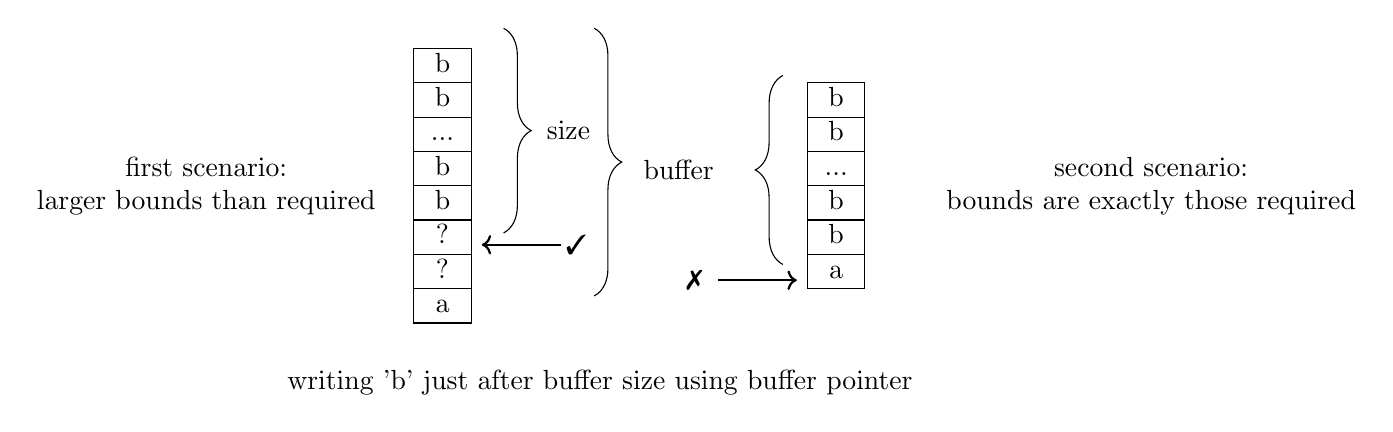
\begin{tikzpicture}
			% Define the data for the array
			\node (array) at (0, 0) {
				\begin{tabular}{|c|}
					\hline
					b \\ \hline
					b \\ \hline
					... \\ \hline
					b \\ \hline
					b \\ \hline
					a \\ \hline
					\end{tabular}
			};
			\node (array) at (-5, 0) {
				\begin{tabular}{|c|}
					\hline
					b \\ \hline
					b \\ \hline
					... \\ \hline
					b \\ \hline
					b \\ \hline
					? \\ \hline
					? \\ \hline
					a \\ \hline
					\end{tabular}
			};
			\node[align=center] at (-8, 0) {first scenario:\\ larger bounds than required};
			\node[align=center] at (4, 0) {second scenario:\\ bounds are exactly those required};

			% Draw the pointer arrow
			\draw[->, thick] (-1.5, -1.2) -- (-0.5, -1.2);
			\node[align=center] at (-1.8, -1.2) {\xmark};

			\draw[->, thick] (-3.5, -0.75) -- (-4.5, -0.75);
			\node[align=center] at (-3.3, -0.75) {\cmark};

			% Add the text for the pointer
			\node at (-3, -2.5) {writing 'b' just after buffer size using buffer pointer};
			\draw [decorate,decoration={brace,amplitude=10pt,raise=5pt}] (-0.5, -1) -- (-0.5, 1.4) node [black,midway,xshift=-1.5cm] {buffer};
			\draw [decorate,decoration={brace,amplitude=10pt,raise=5pt}] (-3.25, 2) -- (-3.25, -1.4) node [black,midway,xshift=-1.5cm] {};
			\draw [decorate,decoration={brace,amplitude=10pt,raise=5pt}] (-4.4, 2) -- (-4.4, -0.6) node [black,midway,xshift=1cm] {size};

		\end{tikzpicture}
	\end{center}
	\textbf{Take a moment to read the following code and comments}
	\lstinputlisting[numbers=none, firstline=7, lastline=40, caption=]{code/ex3-buffer-overflow-global.c}



	To compile, use the Makefile present in the github repository of the \href{https://github.com/CTSRD-CHERI/cheri-exercises}{CTSRD-CHERI/cheri-exercises} repository in the following path: src/exercises/buffer-overflow-global/. 
	
	\begin{tcolorbox}[colback=gray!5!white, colframe=gray!75!black, title=Output on a classic \Gls{risc-v} environment (no CHERI Protection)]
	c = c\\
	c = b
	\end{tcolorbox}
	Here the overflow happens, and the 'c' character is replaced by a 'b'.\break

	\begin{tcolorbox}[colback=gray!5!white, colframe=blue!75!black, title=Output On an environment protected by CHERI]
		c = c\\
		In-address space security exception (core dumped)
	\end{tcolorbox}
	With CHERI protection active, the overflow is detected and prevented.
	Now we will try with 1M+1 byte of buffer size:
	\begin{tcolorbox}[colback=gray!5!white, colframe=blue!75!black, title=Output On an environment protected by CHERI]
		c = c\\
		c = c
	\end{tcolorbox}
	Here the bounds compression made that the buffer had in reality more size than allocated, so the overflow didn't left the bounds of the buffer and didn't change the value of the c character.
	To make this certain, we can add the following lines:

	\begin{lstlisting}[caption=Example C Code]
	printf("%#p\n",buffer);
    	printf("%#p\n",&c);
	\end{lstlisting}
	which print:
	\begin{tcolorbox}[colback=gray!5!white, colframe=blue!75!black, title=Output On an environment protected by CHERI]
	0x131000 [rwRW,0x131000-0x225300]\\
	0x225300 [rwRW,0x225300-0x225301]
	\end{tcolorbox}
	So as expected the size of the character c is 1 byte. However the size of the buffer is 1000192 byte and not 1000001 byte, which explains why the  overflow happened without error: 1000002 is still in-bounds of the pointer. And we can see that the character c is still outside of the bounds.
	
 

\subsection{Explore Subobject Bounds: Subobject Overflows}
	The objective here is to understand how sub-objects works in CHERI environment.
	By default, all pointers inside an object have the rights to access to the whole object.
	This can be changed using compiler options "-Xclang -cheri-bounds=subobject-safe", such as all components of all structures only has access to themselves. Using pointer logic, the bounds of a pointer to a sub-object are the size of the sub-object and not the size of the object.
	It is possible to call built-in function: \_\_containerof that takes a subobject and return a pointer to the object.
	During the definition of an object its possible to use the flag \_\_subobject\_use\_container\_bounds so that the attribute marked will have the container bounds, even with the compiler option active.
	It is also possible to mark the structure with this flag such as all elements within have access to the whole structure.
	That means its possible to forbid access generally then gives rights to specific structures and attributes.
	On this exercise, we will try to make an overflow on a subobject in three scenario: no CHERI protection, default CHERI protection, CHERI protection with sub-object protection.
	\textbf{Take a moment to read the following code and comments}
	\lstinputlisting[numbers=none, firstline=6, lastline=10, caption=]{code/ex4-subobjects-bounds.c}
	\lstinputlisting[numbers=none, firstline=20, lastline=40, caption=]{code/ex4-subobjects-bounds.c}
	\begin{center}
		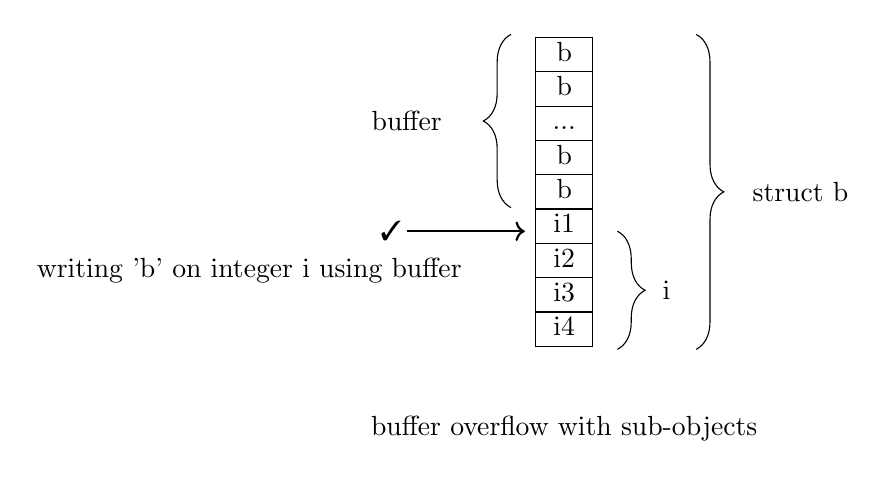
\begin{tikzpicture}
			% Define the data for the array
			\node (array) at (0, 0) {
				\begin{tabular}{|c|}
					\hline
					b \\ \hline
					b \\ \hline
					... \\ \hline
					b \\ \hline
					b \\ \hline
					i1 \\ \hline
					i2 \\ \hline
					i3 \\ \hline
					i4 \\ \hline
					\end{tabular}
			};
		
			% Draw the pointer arrow
			\draw[->, thick] (-2, -0.5) -- (-0.5, -0.5);
			% Add the text for the pointer
			\node at (-4, -1) {writing 'b' on integer i using buffer};
			\draw [decorate,decoration={brace,amplitude=10pt,raise=5pt}] (-0.5, -0.2) -- (-0.5, 2) node [black,midway,xshift=-1.5cm] {buffer};
			\draw [decorate,decoration={brace,amplitude=10pt,raise=5pt}] (0.5, -0.5) -- (0.5, -2) node [black,midway,xshift=0.8cm] {i};
			\draw [decorate,decoration={brace,amplitude=10pt,raise=5pt}] (1.5, 2) -- (1.5, -2) node [black,midway,xshift=1.5cm] {struct b};
			\node at (0, -3) {buffer overflow with sub-objects};
			\node at (-2.2, -0.5) {\cmark};

		\end{tikzpicture}
	\end{center}





	To compile, use the Makefile present in the github repository of the \href{https://github.com/CTSRD-CHERI/cheri-exercises}{CTSRD-CHERI/cheri-exercises} repository in the following path: src/exercises/subobject-bounds/. 
	This will produce following results:
	\begin{tcolorbox}[colback=gray!5!white, colframe=gray!75!black, title=Output on a classic \Gls{risc-v} environment (no CHERI Protection)]
	b.i = c\\
	b.i = b
	\end{tcolorbox}
	\begin{tcolorbox}[colback=gray!5!white, colframe=blue!75!black, title=Output On an environment protected by CHERI]
		b.i = c\\
		b.i = b
	\end{tcolorbox}
	Which are the same. By default CHERI subobject have access to the whole structure, meaning their bonds are those of the structure, meaning that buffer can write over integer i. Now, we will compile the CHERI program with the compiler option "-Xclang -cheri-bounds=subobject-safe".
	The execution results changes:
	\begin{tcolorbox}[colback=gray!5!white, colframe=blue!75!black, title=Output On an environment protected by CHERI \& Subobject Protection]
		b.i = c\\
		In-address space security exception (core dumped)
	\end{tcolorbox}
	The overflow was detected and prevented, because the bounds of the subobjects are exactly their size, meaning that when the buffer tries to write over integer i, it cannot due to his bounds.
	


\subsection{Explore Subobject Bounds: Subobject Overflows}

The code can be found in this \href{https://ctsrd-cheri.github.io/cheri-exercises/exercises/subobject-bounds/}{repository}.
The following image comes from \href{https://ctsrd-cheri.github.io/cheri-exercises/exercises/subobject-bounds/subobject-bounds.pptx}{exercises presentation}.
\begin{figure}
\begin{minipage}{\linewidth}
	\includegraphics[width=\linewidth]{images/Lists-explanations.png}
\end{minipage}
\caption{Linked List}
\end{figure}
In order to make things appear simple, we split the code into three parts:
The linked list structure:
\lstinputlisting[numbers=none, firstline=14, lastline=18, caption=]{code/ex4-lists.c}
The object, a value and a node of the linked list structure.
\lstinputlisting[numbers=none, firstline=52, lastline=60 caption=]{code/ex4-lists.c}
The creation of the object list.
\lstinputlisting[numbers=none, firstline=66, lastline=70, caption=]{code/ex4-lists.c}


As this exercises uses things that requires CHERI to be active (access to capability bounds), we will begin directly with CHERI protected environment.
\begin{tcolorbox}[colback=gray!5!white, colframe=blue!75!black, title=Output On an environment protected by CHERI]
	Traversing list=0x131060 [rwRW, 0x131060-0x131080] \\
	first=0x130f40 [rwRW,0x130f30-0x130f60] lastnp=0x130fb0 [rwRW, 0x130f90-0x130fc0]\\
	Ilist cursor=0x130f40 [rwRW, 0x130f30-0x130f60]\\
	next=0x130fa0 [rwRW, 0x130f90-0x130fc0]\\
	prevnp=0x131070 [rwRW,0x131060-0x131080]\\
	val field at 0x130f30 [rwRW, 0x130f30-0x130f60]\\
	Ilist cursor=0x130fa0 [rwRW, 0x130f90-0x130fc0]\\
	next=0x131060 [rwRW, 0x131060-0x131080]\\
	prevnp=0x130f50 [rwRW, 0x130f30-0x130f60]\\
	val field at 0x130f90 [rwRW, 0x130f90-0x130fc0]\\
	Traversing list again, accessing superobject field\dots\\
	Ilist cursor=0x130f40 [rwRW, 0x130f30-0x130f60] value=1 (at 0x130f30 [rwRW,0x130f30-0x130f60])\\
	Ilist cursor=0x130fa0 [rwRW, 0x130f90-0x130fc0] value=3 (at 0x130f90 [rwRW, 0x130f90-0x130fc0])
\end{tcolorbox}

This exercise uses a chain-list to demonstrate why subobject are not protected by default.\\
To avoid some confusion remember that when printing a pointer, it prints the address of the pointed value and the bounds of the pointed structure. Not those of the object containing the pointer. Which means printing a pointer in an object is useful to see the bounds of the pointed object, not the bounds of the object including the pointer that is printed.
The list is composed of three elements :\\

The sentinel which is a struct of two pointers : one pointing on the first object of the list, one on the next pointer of the last object (the next pointer of the last object lead to the sentinel next pointer but that is not the purpose of next pointer because they have access to the whole structure by default, allowing modifying value or list pointers) it is two pointers so 32 bytes : 20 in hexadecimal, so this explains the given bounds [0x131060-0x131080] we know thanks to the first element previous next pointer that the next pointer of the sentinel is on 0x131070 which means that the next pointer of the sentinel occupies this space : 0x131070-0x131080, due to the fact pointer in CHERI architecture occupies 16 bytes and that the previous next pointer of the sentinel which leads to the last object next pointer of the list, is on this space : 0x131060-0x131070.\\
The first object which is a struct of three pointers : one pointing at the object value, one pointing at the next element of the list (which is the third because the second was removed) and which bounds are (0x130f60-0x130f90) because the pointer of the list element points on the next list element which is different from the object in the list, but still at the same memory space, because there’s one more pointer in the object (the value pointer)(an object is a list element and a value, a list element is a next pointer and a previous next pointer), for this object : we know thanks to the second object previous next pointer that the next pointer of the first object is on 0x130f50 and the bounds of the first object are 0x130f30-0x130f60 which means that the object value pointer is on 0x130f50-0x130f60, the cursor indicate us the position of the element in list which corresponds to the next pointer of the first object which we can place on 0x130f40-0x130f50, the only pointer that remains is the value pointer which is on 0x130f30-0x130f40. Which explains the given bounds : 0x130f30-0x130f60\\
The second object which is the third because the true second was removed, is also a struct of three pointers : one pointing at an object value, one pointing at the next element of the list (which is the sentinel, meaning end of list) and one at the previous next pointer which is the next pointer of the first element, leading to this second list element (which is the third, considering the second was removed). We know thanks to the previous next pointer of the sentinel, that the next pointer of the second object is located in 0x130fb0, the cursor indicates the next pointer of the second object on 0x130fa0 which means that on [0x130f90-0x130fa0] there’s the object value pointer, on [0x130fa0-0x130fb0] there’s the next pointer of the second object leading to the sentinel, on [0x130fb0-0x130fc0] there’s the previous next pointer of the second object, pointing on the first object next pointer.\\
So a list element is only composed of a next pointer and a previous next pointer (like the sentinel) but has access to the value pointer which is just before the element list, because the object struct includes the list element struct. A pointer leading to the element list struct of an object has access to whole object because pointer are not protected from inside pointer of a struct, their bounds include the whole struct.\\

When using "-Xclang -cheri-bounds=subobject-safe" compiler option, nothing changes, because in object definition the original code is using "\_\_subobject\_use\_container\_bounds" flag on the ilist element, which allow this subobject to have access to the whole object.
An execution with the compiler  sub-object protection option and the flag removed look like this:
\begin{tcolorbox}[colback=gray!5!white, colframe=blue!75!black, title=Output On an environment protected by CHERI \& Subobject protection]
	Traversing list=0x131060 [rwRW, 0x131060-0x131080] \\
	first=0x130f40 [rwRW,0x130f30-0x130f60] lastnp=0x130fb0 [rwRW, 0x130f90-0x130fc0]\\
	Ilist cursor=0x130f40 [rwRW, 0x130f30-0x130f60]\\
	next=0x130fa0 [rwRW, 0x130f90-0x130fc0]\\
	prevnp=0x131070 [rwRW,0x131060-0x131080]\\
	val field at 0x130f30 [rwRW, 0x130f30-0x130f60]\\
	Ilist cursor=0x130fa0 [rwRW, 0x130f90-0x130fc0]\\
	next=0x131060 [rwRW, 0x131060-0x131080]\\
	prevnp=0x130f50 [rwRW, 0x130f30-0x130f60]\\
	val field at 0x130f90 [rwRW, 0x130f90-0x130fc0]\\
	Traversing list again, accessing superobject field\dots\\
	In-address space security exception (core dumped)
\end{tcolorbox}

This is because pointer of list only have access to the list structures. Remember that the object is different from the list element, it contains one more value. Pointers of the list can be used to navigate from one element to the other without problems (a pointer to next have access to a next pointer which have access to the following next pointer... until the beginning of the list). However they can not be used to access the value (without the flag allowing them to access the whole structure, the value is out of bound).
Which is why it produces the above security exception which is a Capability Bound Fault.


\subsection{Corrupt a control-flow pointer using a subobject buffer overflow}
The code can be found on this \href{https://ctsrd-cheri.github.io/cheri-exercises/exercises/control-flow-pointer}{repository}.
If an overflow can happen in CHERI subobjects, what happen in the case where the overflow modifies a pointer on a function ?
Here we are going to see that if the pointer is modified during the copying, as it is not an authorized modification the validity tag becomes 0 and so the pointer can not be dereferenced, which means the function can not be called. 
\lstinputlisting[numbers=none, firstline=7, lastline=22, caption=]{code/ex5-buffer-overflow-fnptr.c}
\begin{center}
	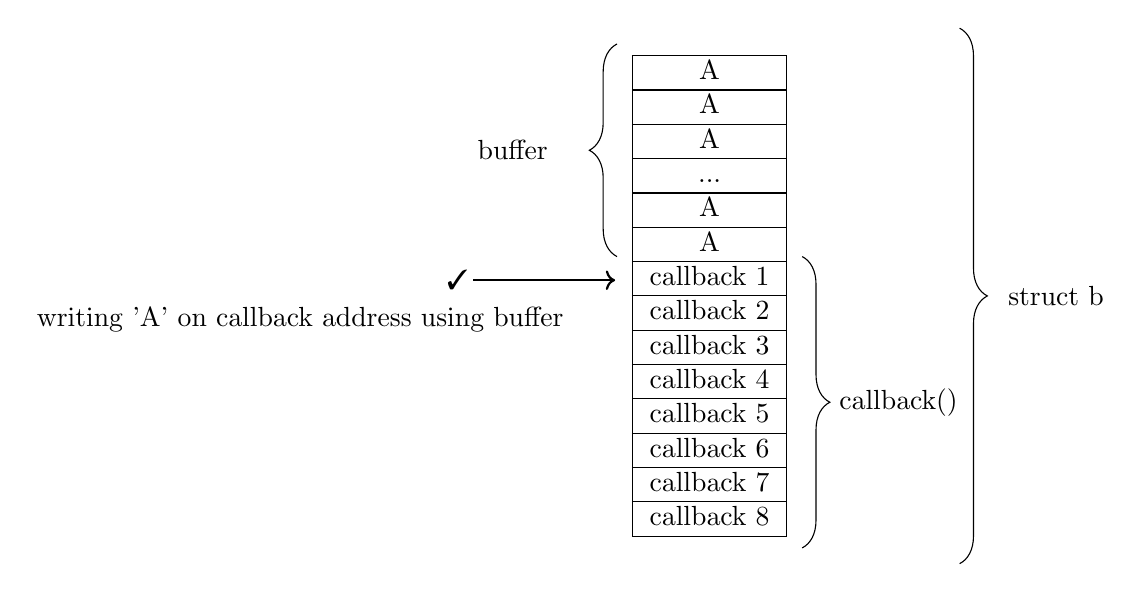
\begin{tikzpicture}
		% Define the data for the array
		\node (array) at (0, 0) {
			\begin{tabular}{|c|c|c|c|c|c|c|c|}
				\hline
				A \\ \hline
				A \\ \hline
				A \\ \hline
				... \\ \hline
				A \\ \hline
				A \\ \hline
				callback 1 \\ \hline
				callback 2 \\ \hline
				callback 3 \\ \hline
				callback 4 \\ \hline
				callback 5 \\ \hline
				callback 6 \\ \hline
				callback 7 \\ \hline
				callback 8 \\ \hline
				\end{tabular}
		};
	
		% Draw the pointer arrow
		\draw[->, thick] (-3, 0.2) -- (-1.2, 0.2);
		% Add the text for the pointer
		\node at (-5.2, -0.3) {writing 'A' on callback address using buffer};
		\draw [decorate,decoration={brace,amplitude=10pt,raise=5pt}] (-1, 0.5) -- (-1, 3.2) node [black,midway,xshift=-1.5cm] {buffer};
		\draw [decorate,decoration={brace,amplitude=10pt,raise=5pt}] (1, 0.5) -- (1, -3.2) node [black,midway,xshift=1.4cm] {callback()};
		\draw [decorate,decoration={brace,amplitude=10pt,raise=5pt}] (3, 3.4) -- (3, -3.4) node [black,midway,xshift=1.4cm] {struct b};
		\node at (-3.2, 0.2) {\cmark};

	\end{tikzpicture}
\end{center}



	Both CHERI environment and not protected CHERI environment produces the same result in this exercise:
	\begin{tcolorbox}[colback=gray!5!white, colframe=gray!75!black, title=Output On both environment]
	Segmentation fault(core dumped)
	\end{tcolorbox}
	This happen because the program tries to call 0xAAAAAAAA as a function. This address is not linked with anything which ends up in segmentation fault.
	Also, in CHERI the segmentation fault has priority over the validity tag. To prove this, we can modify the code like this:


	\begin{lstlisting}[caption=Control flow modified C Code]
		#include <stdint.h>
		---------------------------------
		void test(){
			printf("test\n");
		}
		--------------------------------
		size_t i;
		for (i = 0; i < bp->length; i++){
        	bp->buffer[i] = 0xAAAAAAAA;
		}
        	bp->buffer[i] = (intptr_t)(&test);
	\end{lstlisting}
	With this modification, the error becomes:
	\begin{tcolorbox}[colback=gray!5!white, colframe=blue!75!black, title=Output of modified Code run with CHERI protection ]
		In-address space security exception (core dumped)
	\end{tcolorbox}
	Using gdb, it is possible to obtain more details: 
	\begin{tcolorbox}[colback=gray!5!white, colframe=black!75!black, title=GDB Output of modified Code run with CHERI protection ]
		Program received signal SIGPROT, CHERI protection violation.
		Capability tag fault.
	\end{tcolorbox}
	Which proves that after a not authorized modification of function pointer, the validity tag is put to 0 and throw an error when trying to be dereferenced.
	

\subsection{Exercise heap overflows}
	The code can be found on this \href{https://ctsrd-cheri.github.io/cheri-exercises/exercises/buffer-overflow-heap}{repository}.
	We have seen stack overflows behaviors, what about heap overflow behavior ?
	It has a similar behavior to the stack. However, memory allocation is not always precise which means in some scenarios one could think the code will produce an overflow where in reality, that is not the case.
	\lstinputlisting[numbers=none, firstline=10, caption=]{code/ex6-heap-overflow.c}
\begin{center}
		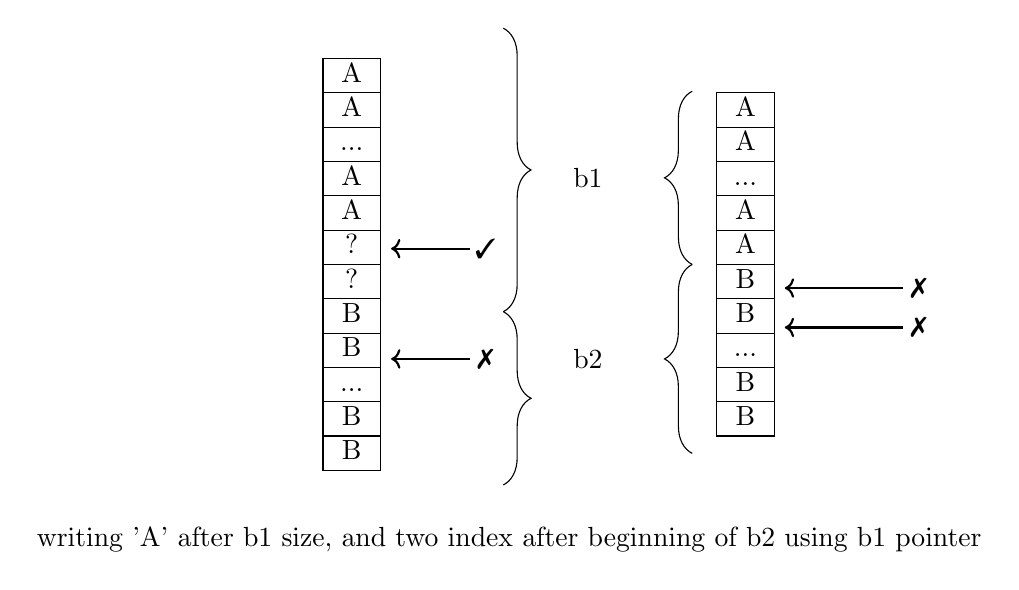
\begin{tikzpicture}
			% Define the data for the array
			\node (array) at (0, 0) {
				\begin{tabular}{|c|}
					\hline
					A \\ \hline
					A \\ \hline
					... \\ \hline
					A \\ \hline
					A \\ \hline
					B \\ \hline
					B \\ \hline
					... \\ \hline
					B \\ \hline
					B \\ \hline
					\end{tabular}
			};
			\node (array) at (-5, 0) {
				\begin{tabular}{|c|}
					\hline
					A \\ \hline
					A \\ \hline
					... \\ \hline
					A \\ \hline
					A \\ \hline
					? \\ \hline
					? \\ \hline
					B \\ \hline
					B \\ \hline
					... \\ \hline
					B \\ \hline
					B \\ \hline
					\end{tabular}
			};
		
			% Draw the pointer arrow
			\draw[->, thick] (2, -0.3) -- (0.5, -0.3);
			\node at (2.2, -0.3) {\xmark};

			\draw[->, thick] (-3.5, 0.2) -- (-4.5, 0.2);
			\node at (-3.3, 0.2) {\cmark};

			\draw[->, thick] (2, -0.8) -- (0.5, -0.8);
			\node at (2.2, -0.8) {\xmark};

			\draw[->, thick] (-3.5, -1.2) -- (-4.5, -1.2);
			\node at (-3.3, -1.2) {\xmark};

			% Add the text for the pointer
			\node at (-3, -3.5) {writing 'A' after b1 size, and two index after beginning of b2 using b1 pointer};

			\draw [decorate,decoration={brace,amplitude=10pt,raise=5pt}] (-0.5, 0) -- (-0.5, 2.2) node [black,midway,xshift=-1.5cm] {b1};
			\draw [decorate,decoration={brace,amplitude=10pt,raise=5pt}] (-3.25, 3) -- (-3.25, -0.6) node [black,midway,xshift=-1.5cm] {};
			\draw [decorate,decoration={brace,amplitude=10pt,raise=5pt}] (-0.5, -2.4) -- (-0.5, 0) node [black,midway,xshift=-1.5cm] {b2};
			\draw [decorate,decoration={brace,amplitude=10pt,raise=5pt}] (-3.25, -0.6) -- (-3.25, -2.8) node [black,midway,xshift=-1.5cm] {};

		\end{tikzpicture}
	\end{center}	




	
		This program requires an argument to run, otherwise it will throw an assertion error. 0x20 is a valid argument.
		\begin{tcolorbox}[colback=gray!5!white, colframe=gray!75!black, title=Heap Overflow with 0x20 as parameter without CHERI protection]
			b1=0xef429009000 b2=0xef42900920 diff=20\\
			Overflowing by 1\\
			b2 begins: ABBB\\
			Overflowing by 2\\
			b2 begins: AABB
		\end{tcolorbox}
		As we can see, the overflows on the heap are not detected on the normal environment and the buffer characters are being replaced.

		\begin{tcolorbox}[colback=gray!5!white, colframe=blue!75!black, title=Heap Overflow with 0x20 as parameter with CHERI protection]
			b1=0x40c0f000 [rwRW, 0x40c0f000-0x40c0f020] b2=0x40c0f020 [rwRW, 0x40c0f020-0x40c0f040] diff=20\\
			Overflowing by 1\\
			In-address space security exception (core dumped)
		\end{tcolorbox}
		Here the overflow is detected and prevented by the throwing of an error.
		We can use gdb to see the error with more details:
		First, run : "gdb ./buffer-overflow-heap-cheri" then in gdb command line "r 0x20".
		This produces the following error:
		\begin{tcolorbox}[colback=gray!5!white, colframe=black!75!black, title=GDB: Heap Overflow with 0x20 as parameter with CHERI protection]
			b1=0x40c0f000 [rwRW, 0x40c0f000-0x40c0f020] b2=0x40c0f020 [rwRW, 0x40c0f020-0x40c0f040] diff=20\\
			Overflowing by 1\\
			
			Program received signal SIGPROT, CHERI protection violation.\\
			Capability bounds fault.
		\end{tcolorbox}
		Which is coherent because the overflow is an out of bounds.
	
	\subsection{Exercise integer pointer type confusion bug}
	This exercise goal is to prevent programers from using the "long" type to manipulate pointers values, because it is bad practice.  
		To manipulate pointers one must use "intptr\_t" or "uintptre\_t" types, using stdint.h. 
		\lstinputlisting[numbers=none, firstline=9, lastline=12, caption=]{code/ex7-integer-pointer-type-confusion-bug.c}
		hello is a pointer that reference the string "Hello World". 
		\lstinputlisting[numbers=none, firstline=23, lastline=28, caption=]{code/ex7-integer-pointer-type-confusion-bug.c}

		This code can be found on this \href{https://ctsrd-cheri.github.io/cheri-exercises/exercises/type-confusion/}{repository}.
    
	
		Even if cast from long to pointer work in standard environment, it is not a good practice to use it.
		\begin{tcolorbox}[colback=gray!5!white, colframe=gray!75!black, title=Output on classic \Gls{risc-v} environment (No CHERI protection)]
			lp.ptr Hello World!\\
			lp.ptr ello World!
		\end{tcolorbox}
		\begin{tcolorbox}[colback=gray!5!white, colframe=blue!75!black, title=Execution on CHERI environment]
			lp.ptr Hello World!\\
			In-address space security exception (core dumped)
		\end{tcolorbox}
		Under CHERI protections, it can not be cast to a pointer and produce a security exception.
		The long is supposed to be use for great precision numbers. Not to be cast to a pointer.
		In CHERI, using long for pointer is problematic because of validity tag. A variable of type intptr\_t will have its validity tag in memory which means that if it is modified by not authorized operation, the pointer obtained from a potential cast will be not valid.
		However if CHERI allowed long conversion, either it creates a validity tag for each long, even if they are not supposed to be pointers, or a modification of a long could in a non authorized way result in a valid pointer, which would go against the spacial property of CHERI.
		You can test this by doing a buffer overflow on a intptr\_t variable and try to dereferenced it after cast to pointer.
	
	\subsection{Demonstrate pointer injection}
		This exercise goal is to demonstrate that CHERI forbid pointer use, if the pointer comes from another process.
		First is an example of sharing raw value that works. The code can be found on this \href{https://ctsrd-cheri.github.io/cheri-exercises/exercises/pointer-injection/index.html}{repository}.
	
	
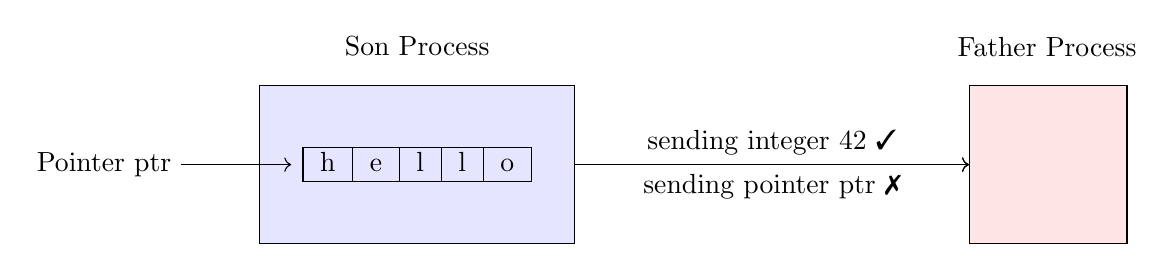
\begin{tikzpicture}
	\node[draw, fill=blue!10, minimum height=2cm, minimum width=4cm] (rect1) {
		\begin{tabular}{|c|c|c|c|c|}
			\hline
			h & e & l & l & o \\
			\hline
			\end{tabular}
		};

	   \node[draw, fill=red!10, right=5cm of rect1, minimum height=2cm, minimum width=2cm] (rect2) {};
	   \draw[->] (rect1.east) -- node[above] {sending integer 42 \cmark} (rect2.west);
	   \draw[->, yshift=-1cm] (rect1.east) -- node[below] {sending pointer ptr \xmark} (rect2.west);
   	   \node[left=3cm] (pointer) {Pointer ptr};
	   \draw[->] (pointer.east) -- ++(1.4,0);
	   \node at (0, 1.5) {Son Process};
	   \node at (8, 1.5) {Father Process};

\end{tikzpicture}
	
		\lstinputlisting[numbers=none, firstline=12, lastline=33, caption=]{code/long-over-pipe.c}
		Second is an example of sharing a pointer that will fail under CHERI protection.
		\lstinputlisting[numbers=none, firstline=9, lastline=39, caption=]{code/ptr-over-pipe.c}
	
	
		The program is not very verbose. Here is what it does: it forks, creating one more process. One process will then send data to the other one using a pipe.
		\begin{tcolorbox}[colback=gray!5!white, colframe=blue!75!black, title=Execution of long transmission on CHERI environment]
			received 42
		\end{tcolorbox}
		\begin{tcolorbox}[colback=gray!5!white, colframe=blue!75!black, title=Execution of ptr transmission on CHERI environment]
			In-address space security exception (core dumped)
		\end{tcolorbox}
		When a process give an address to another process, the received pointer is not valid, which means it can not be dereferenced. Trying to do so throw the above security exception.
	
	\subsection{Adapt C Program to CHERI C}
		The objective of this exercise is to learn how to adapt C programs, using gdb to identify the faulting lines of code.
		The code is quite long so we are not going to print it in this explanations.
		The makefile is not correct in this exercise. Here is an explanation to how compile:
		cc -c methods.c ; 
		cc -o cat cat.c methods.o
		CHERI compiler will warn about the things that are problematic. In order to do the exercise properly you must ignore the warnings and try to execute the code directly, it will not work, then you will have to debug using gdb to found out that the problems were the things the compiler warned you about.
		The program is cat, which means it takes an argument corresponding to a file you want to print.
		If you don't know what to print, just use the c program.
		The code can be find \href{https://ctsrd-cheri.github.io/cheri-exercises/exercises/adapt-c/index.html}{here}.
	
	
	 In order to run the program and execute it step by step, you can do "break main" then "r" then "nexti" until it crashes.
	 After finding the section of code that is throwing the error, which is normally a function call, you can step into it using "stepi" after running again the program. This will aid you to find the problematic section.
	 It is possible to place breakpoints on the function calls of problematic warnings mentioned in compiler.
	 Another option is to have read the code and seen that "write(2) failed" is an error thrown in raw\_cat function, when write\_off function fails and place break point on write\_off.
	 write\_off function uses a cast to const void* of an offset and a buffer. The problem is that CHERI must know what is a pointer and what is an offset in order to conserve bounds and validity tag. Here the cast from buf to uintptr\_t confuse the compiler because it has two pseudo pointer values to add.
	 One way to solve the situation is to remove the cast to uintptr\_t on buf, that way we add a pointer and an offset and the compiler is not confused.
	 The other problem comes of long variable which is then cast to FILE * (a pointer). And as we know this very bad practice is not allowed on CHERI which causes the program to crash.
	 So we must modify the function prototype like this: static void verbose\_cat(intptr\_t file). It will work. But to do it properly, this is a little more complex as now we have to modify everything related to this function (the function call and variable used in it).
		

	\subsection{CHERIABI Showcase | Kernel confuse deputy problem}

		The kernel confuse deputy is a potential problem that could happen when doing a system call, because the program let the kernel do operations. The problem is that the kernel has all rights on memory. Which means something with limited rights could potentially have access to other things it is not supposed to.
		But CHERI uses a pointer in the arguments that gives intention in system calls so that the kernel verify that the pointer with the given intention is not trying to access something it is not supposed to. 

		In this example, there is a fork to create a second process, then one process will send integers that will be put in an array (which itself is an allowed operation), the problem is that the number of sent integer is superior to the size of the array.
		This example can be find \href{https://ctsrd-cheri.github.io/cheri-exercises/exercises/cheriabi/index.html}{here}.
		\begin{center}
			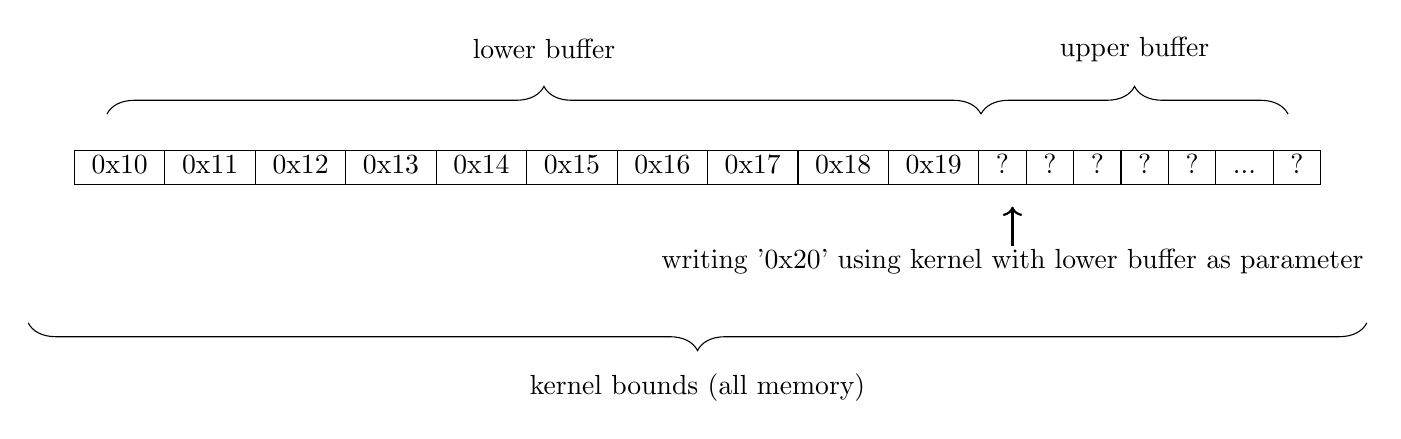
\begin{tikzpicture}
				\node (array) at (0, 0) {
					\begin{tabular}{|c|c|c|c|c|c|c|c|c|c|c|c|c|c|c|c|c|}
						\hline
						0x10 & 0x11 & 0x12 & 0x13 & 0x14 & 0x15 & 0x16 & 0x17 & 0x18 & 0x19 & ? & ? & ? & ? & ? & ... & ?\\ \hline
					\end{tabular}
				};
			
				\draw[->, thick] (4, -1) -- (4, -0.5);
				\node at (4, -1.2) {writing '0x20' using kernel with lower buffer as parameter};
				\draw [decorate,decoration={brace,amplitude=10pt,raise=5pt}] (-7.5, 0.5) -- (3.6, 0.5) node [black,midway,yshift=1cm] {lower buffer};
				\draw [decorate,decoration={brace,amplitude=10pt,raise=5pt}] (3.6, 0.5) -- (7.5, 0.5) node [black,midway,yshift=1cm] {upper buffer};
				\draw [decorate,decoration={brace,amplitude=10pt,raise=5pt}] (8.5, -1.8) -- (-8.5, -1.8) node [black,midway,yshift=-1cm] {kernel bounds (all memory)};

			\end{tikzpicture}
		\end{center}	\lstinputlisting[numbers=none, firstline=20, lastline=58, caption=]{code/ex8-kern-read-over.c}
	
	
	
	
		In a standard execution environment, overflows happen without kernel intervention, so its not surprising to see the overflow was not detected.
		\begin{tcolorbox}[colback=gray!5!white, colframe=gray!75!black, title=Output on classic \Gls{risc-v} environment (No CHERI protection)]
			Write OK\\
			lower=0x802cbe30 upper=0x802cbe40\\
			Read 0x20; lower[0]=0x10 upper[0]=0x20
		\end{tcolorbox}
		\begin{tcolorbox}[colback=gray!5!white, colframe=blue!75!black, title=Output on CHERI protected environment]
			Write OK\\
			lower=\ptraddress{}7ff00 upper=\ptraddress{}f7ff10\\
			Bad read (Bad address); lower[0]=0x10 upper[0]=0x0
		\end{tcolorbox}
		Here the kernel realize that an operation is suspicious and end with a return error value. This is different from a security exception.
		It stops before writing on upper buffer but lower buffer has been modified and the program can continue after the error is returned.
	
	\subsection{CHERIABI Showcase | Memory mapping process}
		I modified the original code to add more prints, to understand the problem better. The code will allocate in various authorized ways then try to map on a memory zone that is already allocate.
		I didn't understand all subtleties of this exercise so i will not try to explain in details what happen.
		Its possible to use \_\_builtin\_cheri\_perms\_get built in function to access rights of pointer. 
		We use same print convention as first exercise: PRINTF\_PTR stands for \%p for normal prints and <\%\#p for execution under CHERI environment.
		\lstinputlisting[numbers=none, firstline=21, caption=]{code/ex8-perm-vmem.c}
	
	
	
		One important thing to notice is that the two first mappings, are located at the same address (somewhere in anonymous memory). The second one is mapped after the first one is freed.
		The third allocation is on the heap and is not deallocated.
		For the fourth allocation, the program tries to allocate something already allocated (mapping directly into the heap).
		\begin{tcolorbox}[colback=gray!5!white, colframe=gray!75!black, title=Output on classic \Gls{risc-v} environment (No CHERI protection)]
			Directly mapped page at p=0x78e42a200000\\
			Directly mapped page at p=0x78e42a200000\\
			allocate memory using malloc at m=0x78e429c13000\\
			Punching hole in the heap at p=0x78e429c13000\\
			Directly mapped page at p=0x78e429c13000\\
			Done
		\end{tcolorbox}
		\begin{tcolorbox}[colback=gray!5!white, colframe=blue!75!black, title=Output on CHERI protected environment]
			Directly mapped page at p=0x40821000 [rwRW,0x40821000-0x40822000] p.perms=0x3717d\\
			Directly mapped page at p=0x40821000 [rwRW,0x40821000-0x40822000]\\
			allocate memory using malloc at m=0x40c19000 [rwRW,0x40c19000-0x40c1b000]\\
			Punching hole in the heap at p=0x40c19000 [rwRW,0x40c19000-0x40c1b000]\\
			p.perms=0x37175\\
			Assertion failed: (q != MAP\_FAILED), function main, file perm-vmem.c, line 57.\\
			Abort trap (core dumped)
		\end{tcolorbox}
		\begin{center}
		

			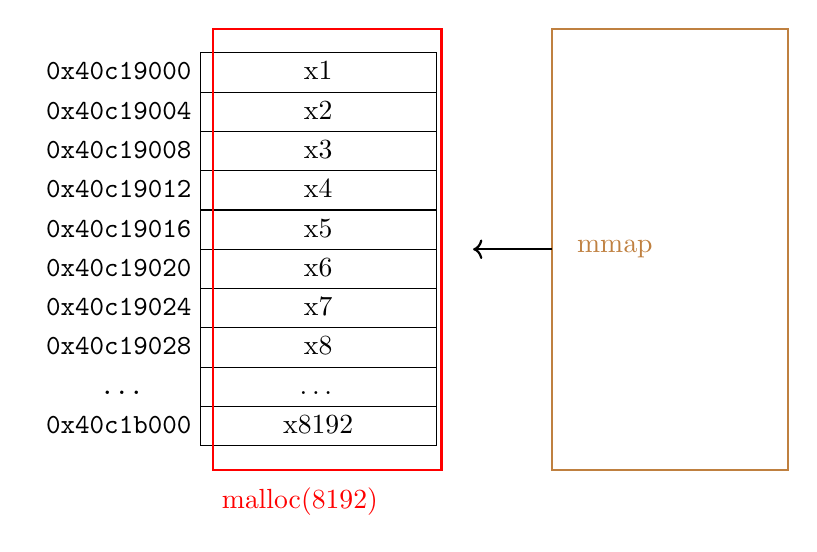
\begin{tikzpicture}
				% Draw the memory table
				\matrix (m) [matrix of nodes,
							 nodes in empty cells,
							 nodes={draw, anchor=center, text height=1.5ex, text depth=.25ex, minimum width=2cm},
							 column 1/.style={nodes={draw=none, anchor=east, minimum width=2cm}},
							 column 2/.style={nodes={draw, anchor=center, minimum width=3cm}},
							 row sep=-\pgflinewidth, column sep=-\pgflinewidth] {
					\texttt{0x40c19000} & x1 \\
					\texttt{0x40c19004} & x2 \\
					\texttt{0x40c19008} & x3 \\
					\texttt{0x40c19012} & x4 \\
					\texttt{0x40c19016} & x5 \\
					\texttt{0x40c19020} & x6 \\
					\texttt{0x40c19024} & x7 \\
					\texttt{0x40c19028} & x8 \\
					\texttt{...} & \ldots \\
					\texttt{0x40c1b000} & x8192 \\
				};
		

				\draw[red, thick] (-0.3,2.8) rectangle (2.6,-2.8); 

				\draw[brown, thick] (4,2.8) rectangle (7,-2.8);
				\draw[->, thick] (4, 0) -- (3, 0);
				\node[text=red] at (0.8, -3.2) {malloc(8192)};
				\node[text=brown] at (4.8, -0) {mmap};

			\end{tikzpicture}
		\end{center}
		The mapping fail under CHERI protection, returning MAP\_FAILED. The error is then thrown by an assertion. Meaning that it would be possible to continue code execution (potentially try catching the error).
		The exercise goal is to show that with CHERI protection, its not possible to use mapping to access unauthorized memory zone (including already allocated memory zone).
	

	\subsection{Extending heap allocators for CHERI}

		This exercise uses a simple example to illustrate a more complex problem.
		The more global problem is related to temporal and spacial safety, on allocation, metadata manipulation and memory freeing. Its common practice in C to stock metadata outside of an object.
		However in CHERI this practice can not be allowed, as it would be out the bounds of the object, which means the object must include meta-data, that could be implemented by augmentation of pointer bounds when necessary (its possible to dynamically modify the bounds of a pointer).
		In the following code is implemented a simple version of an allocator with fixed size and no metadata.
		This allocator will be itself allocated as an array of a specific structure and then when a specific function is called, "allocate" memory to pointers, using byte arrays.
		As the arrays of structure are allocated together, they follow each other on the memory, meaning that a buffer overflow on byte array might have impact on the next structure.
		The allocator uses a pointer named alloc\_next\_free to identify the next free byte array. However to actualize this pointer, the program uses the next pointer. Which means overflowing at a memory allocation will not stop the allocator from allocating the corrupted structure instance, but it will produce an error after trying to allocate from this corrupted instance.
		\begin{center}

			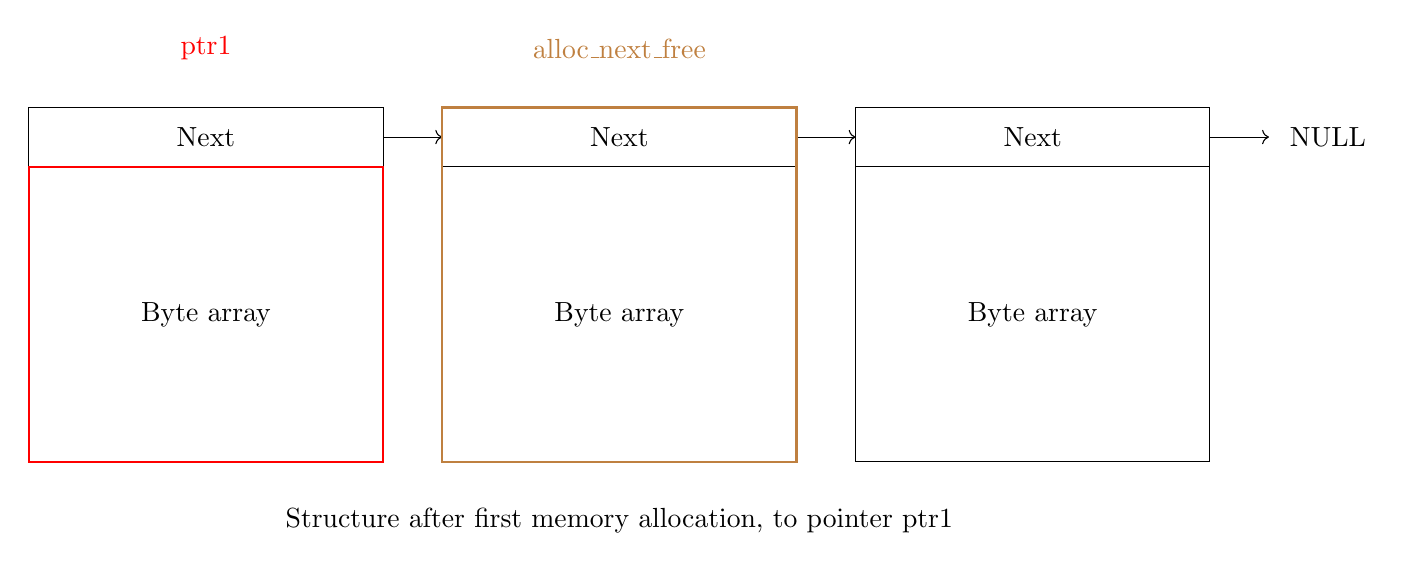
\begin{tikzpicture}[scale=0.75]
			\node at (0,0) {Structure after first memory allocation, to pointer ptr1};
			% First node
			\listnode{-10}{1}{0}
			\listnode{-3}{1}{0}
			\listnode{4}{1}{1}
			\draw[red, thick] (-10,1) rectangle (-4,6); 
			\node[text=red] at (-7, 8) {ptr1};
			\draw[brown, thick] (-3,1) rectangle (3,7); 
			\node[text=brown] at (0, 8) {alloc\_next\_free};
			\end{tikzpicture}
		
			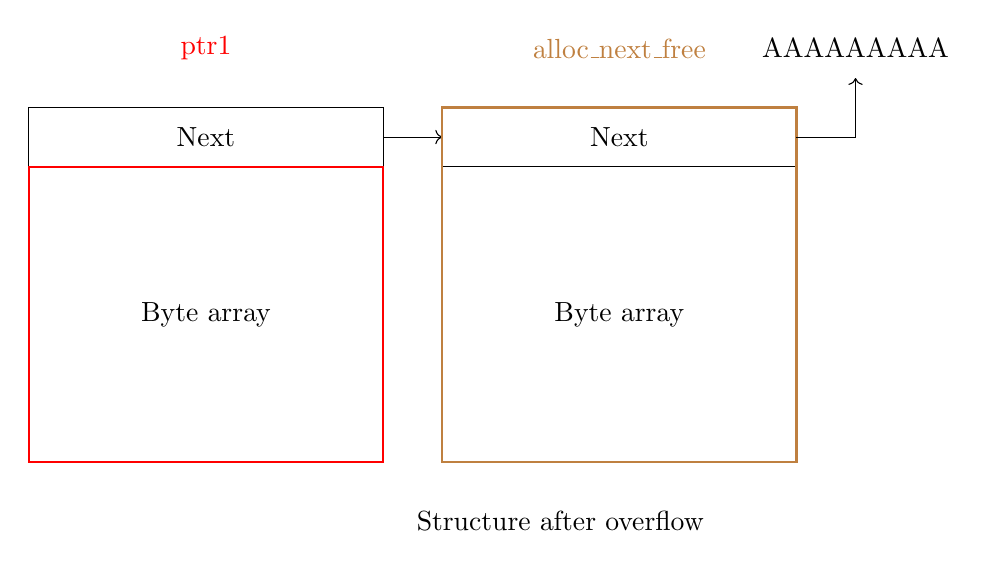
\begin{tikzpicture}[scale=0.75]
			\node at (-1,0) {Structure after overflow};
			% First node
			\allocStorageStruct{-3}{1}		
			\listnode{-10}{1}{0}
			\draw[red, thick] (-10,1) rectangle (-4,6); 
			\node[text=red] at (-7, 8) {ptr1};
			\draw[brown, thick] (-3,1) rectangle (3,7); 
			\draw[->] (3, 6.5) -- (4, 6.5)-- (4, 7.5);
			\node at (4,8) {AAAAAAAAA};
			\node[text=brown] at (0, 8) {alloc\_next\_free};

			\end{tikzpicture}
			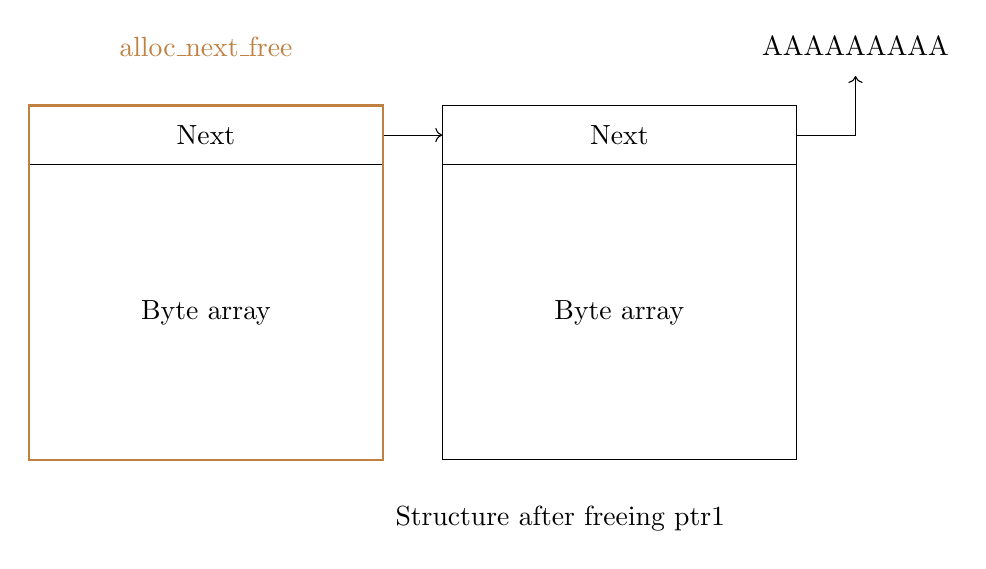
\begin{tikzpicture}[scale=0.75]
				\node at (-1,0) {Structure after freeing ptr1};
				% First node
				\allocStorageStruct{-3}{1}		
				\listnode{-10}{1}{0}
				\draw[brown, thick] (-10,1) rectangle (-4,7); 
				\draw[->] (3, 6.5) -- (4, 6.5)-- (4, 7.5);
				\node at (4,8) {AAAAAAAAA};
				\node[text=brown] at (-7, 8) {alloc\_next\_free};
	
			\end{tikzpicture}

			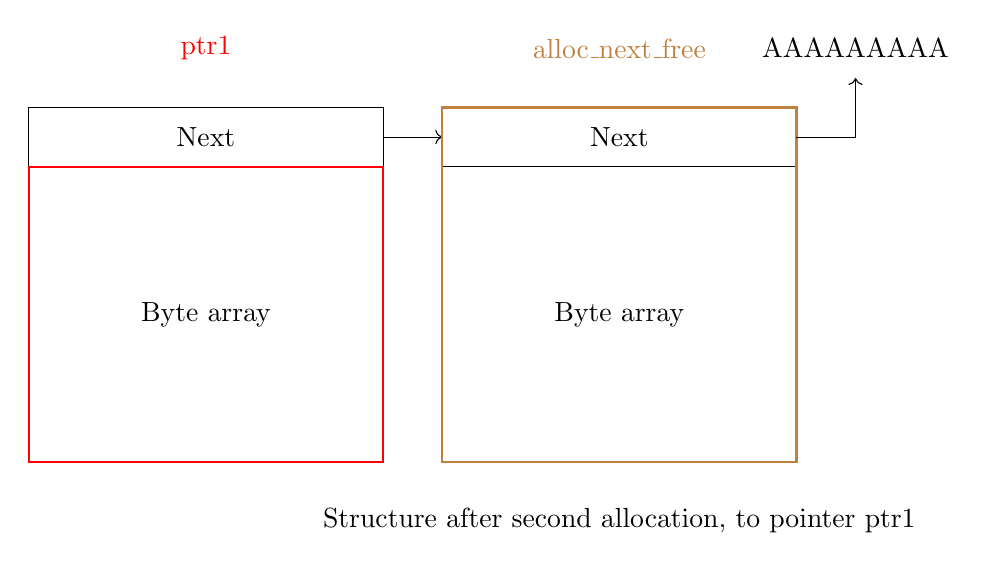
\begin{tikzpicture}[scale=0.75]
				\node at (0,0) {Structure after second allocation, to pointer ptr1};
				% First node
				\allocStorageStruct{-3}{1}		
				\listnode{-10}{1}{0}
				\draw[red, thick] (-10,1) rectangle (-4,6); 
				\node[text=red] at (-7, 8) {ptr1};
				\draw[brown, thick] (-3,1) rectangle (3,7); 
				\draw[->] (3, 6.5) -- (4, 6.5)-- (4, 7.5);
				\node at (4,8) {AAAAAAAAA};
				\node[text=brown] at (0, 8) {alloc\_next\_free};
			\end{tikzpicture}

			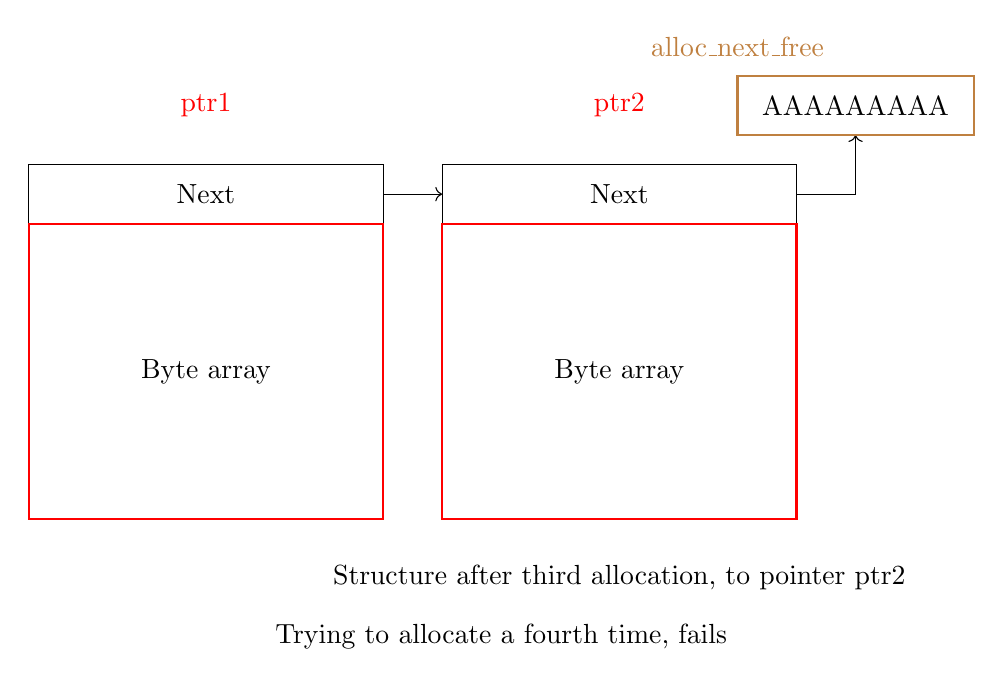
\begin{tikzpicture}[scale=0.75]
				\node at (0,0) {Structure after third allocation, to pointer ptr2};
				% First node
				\allocStorageStruct{-3}{1}		
				\listnode{-10}{1}{0}
				\draw[red, thick] (-10,1) rectangle (-4,6); 
				\node[text=red] at (-7, 8) {ptr1};
				\draw[red, thick] (-3,1) rectangle (3,6); 
				\draw[->] (3, 6.5) -- (4, 6.5)-- (4, 7.5);
				\node at (4,8) {AAAAAAAAA};
				\node[text=red] at (0, 8) {ptr2};

				\draw[brown, thick] (2,7.5) rectangle (6,8.5); 
				\node[text=brown] at (2, 9) {alloc\_next\_free};
				\node at (-2,-1) {Trying to allocate a fourth time, fails};

			\end{tikzpicture}
				
		\end{center}
		

		

		\lstinputlisting[numbers=none, firstline=45, lastline=53, caption=]{code/ex9-heap-allocator.c}
		\lstinputlisting[numbers=none, firstline=120, lastline=170, caption=]{code/ex9-heap-allocator.c}

		This code can be found \href{https://ctsrd-cheri.github.io/cheri-exercises/exercises/cheri-allocator/index.html}{here}.


	
		As this code include CHERI specific code, we can not compile it in a classic environment. We will only take a look at the CHERI execution environment output.
		This allocator functions like a linked list. During execution of program, the address of the next pointer is replaced with 'A' characters.
		\begin{tcolorbox}[colback=gray!5!white, colframe=blue!75!black, title=Output On an environment protected by CHERI]
			Allocator initialised\\
			Allocating memory\\
			Allocation returned 0x131230\\
			Preparing to overflow 0x131230\\
			Overflowed allocation 0x131230\\
			freeing allocation 0x131230\\
			Allocation 0x131230 freed\\
			Allocating memory\\
			Allocation returned 0x131230\\
			Allocating memory\\
			Allocation returned 0x1312c0\\
			Allocating memory\\
			In-address space security exception (core dumped)
		\end{tcolorbox}

		We can look into gdb for more precision:
		\begin{tcolorbox}[colback=gray!5!white, colframe=black!75!black, title=GDB Debug]
			Program received signal SIGPROT, CHERI protection violation.
			Capability tag fault.
		\end{tcolorbox}
		This occurs here: "alloc\_nextfree = alloc->a\_next;"
		\lstinputlisting[numbers=none, firstline=75, lastline=86, caption=]{code/ex9-heap-allocator.c}

		in function alloc\_allocate().
		This is because the previous overflow on the bytes array has replaced the value of the pointer next with 'A' in a not authorized way, meaning that the capability tag was put to 0.
		We can use the function: "cheri\_bounds\_set" to set suitable bounds to the bytes array: it has no reason to access the whole structure.
		Then the overflow is detected as soon as it happen, the error becomes a bounds fault.
		\lstinputlisting[numbers=none, firstline=89, lastline=94, caption=]{code/ex9-heap-allocator.c}

		However this causes the free function to crash: \_\_containerof take as argument a pointer to a subobject and return a pointer to the object, but this pointer has the same rights as the subobject.
		Which means that when trying to access the next pointer using the byte array pointer (which we just reduced rights), a capability bounds fault is thrown.
		\lstinputlisting[numbers=none, firstline=102, lastline=115, caption=]{code/ex9-heap-allocator.c}

		To solve this, we must give ptr pointer larger rights using cheri\_address\_set function which requires a pointer, which bounds and capabilities will be granted, and a second argument with the address.
		The only global variable with minimum rights for what we need to do is the alloc\_array (the whole list) and the address we want to use is obviously the one from ptr pointer (we want to access the next pointer of ptr's structure), and to get that address we can use cheri\_get\_address function.
		\newcommand{\objstruct}[3]{
			\node[] at (#1+2.5, #2+1) {arg};
			\node[] at (#1+2.5, #2+3) {fn};
			\node[] at (#1+2.5, #2+4.5) {buf};
			\ifnum#3=1
			\draw (#1, #2) rectangle (#1+5, #2+5);
			\draw (#1, #2) rectangle (#1+5, #2+2);
			\draw (#1, #2) rectangle (#1+5, #2+4);
			\else
			\draw[dotted] (#1, #2) rectangle (#1+5, #2+5);
			\draw[dotted] (#1, #2) rectangle (#1+5, #2+2);
			\draw[dotted] (#1, #2) rectangle (#1+5, #2+4);
			\fi
		}
	\subsection{Demonstrate Pointer Revocation}
		The goal of this exercise is to show properties in relation with temporal safety, some flaws: use of pointer after free and some good feature: quarantine of freed memory.
		\begin{center}
			\begin{tikzpicture}[scale=0.9]
				\objstruct{0}{0}{1}
				\node[] at (-2.5, 2.5) {obj1};
				\draw[->] (-2, 2.5) -- (0, 2.5);
				\draw[->] (4, 3) -- (6, 3);
				\node[] at (6.5, 3) {fn1};
				\draw (-0.5, 5.5) rectangle (5.5, -1.5);
				\node[] at (2.5, -1) {heap memory};
				\node[] at (2.5, 6) {first allocation};
				\node[] at (2.5, -2) {   };
			\end{tikzpicture}
			\begin{tikzpicture}[scale=0.9]
				\objstruct{0}{0}{0}
				\node[brown] at (-2.5, 2.5) {obj1};
				\draw[brown,->] (-2, 2.5) -- (0, 2.5);
				\draw[->] (4, 3) -- (6, 3);
				\node[] at (6.5, 3) {fn1};
				\draw (-0.5, 5.5) rectangle (5.5, -1.5);
				\node[] at (2.5, -1) {heap memory};
				\node[] at (2.5, -2) {freeing obj1 (still has access to structure)};
			\end{tikzpicture}

			\begin{tikzpicture}[scale=0.9]
				\node[] at (-4.5, 6) {first scenario: no temporal safety};
				\objstruct{-7}{0}{1}
				\node[brown] at (-8.5, 2.5) {obj1};
				\node[] at (-8.5, 1) {obj2};
				\draw[->] (-8, 1) -- (-7, 2.5);
				\draw[->] (-3, 3) -- (-0.5, 3);
				\node[] at (0, 3) {fn2};
				\draw[brown,->] (-8, 2.5) -- (-7, 2.5);
				\draw (-7.5, 5.5) rectangle (-1, -1.5);
				\node[] at (-4, -1) {heap memory};
				\node[] at (4.5, 6) {second scenario: temporal safety};
				\objstruct{2}{-6}{1}
				\objstruct{2}{0}{0}
				\draw (1, 5.5) rectangle (8, -6.5);
				\node[] at (4, -0.5) {heap memory};
				\node[brown] at (0, 2) {obj1};
				\node[] at (0, -3) {obj2};
				\draw[brown, ->] (0.5, 2) -- (2, 2);
				\draw[->] (0.5, -3) -- (2, -3);
				\draw[->] (6, 3) -- (8.5, 3);
				\node[] at (9, 3) {fn1};
				\draw[->] (6, -3) -- (8.5, -3);
				\node[] at (9, -3) {fn2};
				\node[] at (-4.5, -2.5) {third scenario: temporal safety + revoke};
				\objstruct{-7}{-9}{1}
				\node[] at (-4.5, -3.5) {heap memory};
				\draw (-7.5, -9.5) rectangle (-1.5, -3);
				\draw[red, ->] (-1, -6) -- (-2, -6);
				\draw[->] (-1, -7) -- (-2, -6);
				\node[red, align=center] at (0, -6) {obj1 \\ (invalid)};
				\node[] at (0, -7) {obj2};
				\draw[->] (-6, -6) -- (-8, -6);
				\node[] at (-9, -6) {fn2};

			\end{tikzpicture}

		\end{center}
		
		\lstinputlisting[numbers=none, firstline=15, caption=]{code/ex10-temporal-control.c}
	
	
		The two behavior here are similar, but not identical, its important to notice that on the first execution environment, the address of first object and second object are equal (they overlap), where in the second execution environment, one is after the other (no common space).
		The code can be found \href{https://ctsrd-cheri.github.io/cheri-exercises/exercises/cheri-allocator/index.html}{here}.
		\begin{tcolorbox}[colback=gray!5!white, colframe=gray!75!black, title=Output on classic \Gls{risc-v} environment (no CHERI Protection)]
			Installing function pointer in obj1 at 0x25a145609000\\
			Demonstrating use after free:\\
			First function: 0x25a145609000\\
			Assigning function pointer through obj2 at 0x25a145609000\\
			Calling function pointer through obj1 (now 0x25a145609000)\\
			First function: 0x25a145609000
		\end{tcolorbox}
		\begin{tcolorbox}[colback=gray!5!white, colframe=blue!75!black, title=Output on CHERI protected environment]
			Installing function pointer in obj1 at 0x40c0f000 [rwRW,0x40c0f000-0x40c0f040]\\
			Demonstrating use after free:\\
			First function: 0x40c0f000 [rwRW,0x40c0f000-0x40c0f040]\\
			Assigning function pointer through obj2 at 0x40c0f040 [rwRW,0x40c0f040-0x40c0f080]\\
			Calling function pointer through obj1 (now 0x40c0f000  [rwRW,0x40c0f000-0x40c0f040])\\
			First function: 0x40c0f000 [rwRW,0x40c0f000-0x40c0f040]
		\end{tcolorbox}
		Here we can see, in classic environment, the memory space was used again after the free of obj1 to allocate obj2, so the first pointer has access to the second pointer memory space. However with CHERI protection active, even if object 1 was freed, obj2 has a different memory address.
		This is because of memory quarantine: If there are valid pointers pointing on a free memory zone, its not possible to allocate this one.
		We can also see that there is a use after free: first function is called using object 1 even if object 1 was already freed by the time of the call.

		We can now use DCAPREVOKE option on compiler which will tell the program that it can access the malloc\_revoke function, which will invalidate all pointers pointing on free memory, allowing re-use of memory space.
		\begin{tcolorbox}[colback=gray!5!white, colframe=purple!75!black, title=Output on CHERI protected environment \& CAPREVOKE compiler option active]
			Installing function pointer in obj1 at 0x40c0f000 [rwRW,0x40c0f000-0x40c0f040]\\
			Demonstrating use after free:\\
			First function: 0x40c0f000 [rwRW,0x40c0f000-0x40c0f040]\\
			Assigning function pointer through obj2 at 0x40c0f000 [rwRW,0x40c0f000-0x40c0f040]\\
			Calling function pointer through obj1 (now 0x40c0f000  [rwRW,0x40c0f000-0x40c0f040]) (invalid)\\
			In-address space security exception (core dumped)
		\end{tcolorbox}
		As expected, the second object is now allocated on the first object memory and the first object pointer became invalid, and so, by attempting to call a function using this pointer, throw a security exception.
		A problem is that if on the construction of the object, some values are not initialized, they will keep the old values.
		This could be problematic if a condition for using an attribute is that the attribute is not null, here if the old value is not null it could produce unexpected behavior.
	

	\subsection{Exploiting a buffer overflow to manipulate control flow}
		The goal of this mission is to observe the behavior of three different environment when faced with a buffer overflow: a baseline \Gls{risc-v} (classic environment), a CHERI-RISC-V environment and a weakened CHERI-RISC-V environment (in which memory allocator fails to pad allocation in respect of bounds compression imprecision).
		The code can be found \href{https://ctsrd-cheri.github.io/cheri-exercises/missions/buffer-overflow-control-flow/index.html}{here}.
		
		\newcommand{\bofigure}[2]{
			\draw (#1, #2) rectangle (#1+5, #2+4);
			\draw (#1, #2) rectangle (#1+5, #2+2);
			\node[] at (#1+2.5, #2+3) {buffer};
			\node[] at (#1+2.5, #2+1) {function pointer};
		}
		\begin{center}
		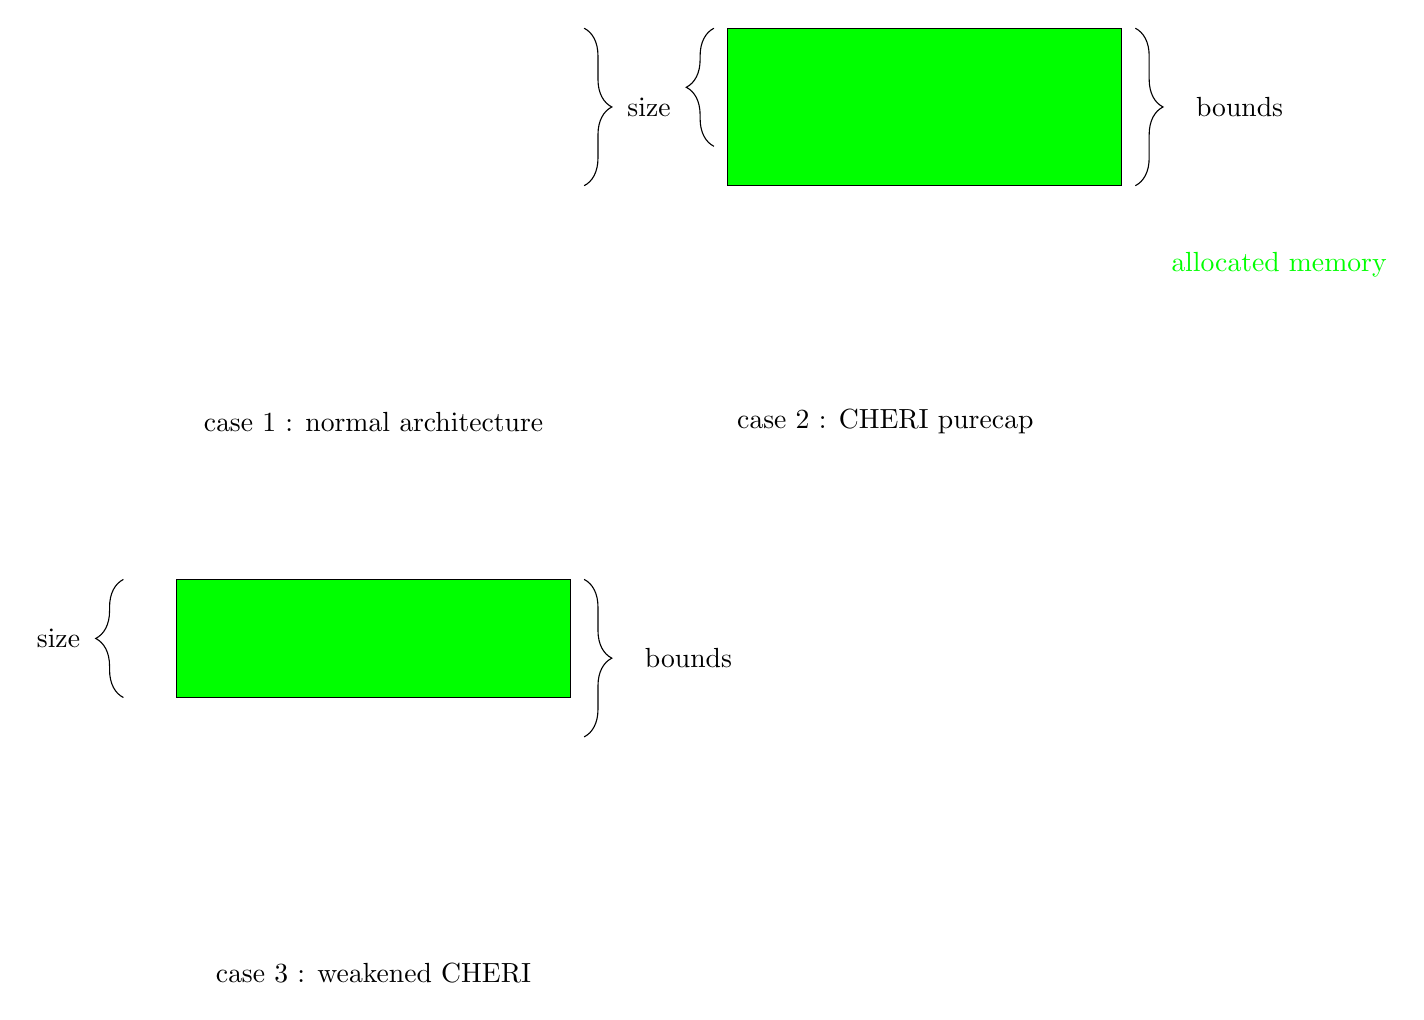
\begin{tikzpicture}
			\draw [fill=green] (7,2) rectangle (12,4);
			\node[green] at (14, 1) {allocated memory};

			\bofigure{0}{0}
			\node[] at (2.5, -1) {case 1 : normal architecture};
			\bofigure{7}{0}
			\node[] at (9, -1) {case 2 : CHERI purecap};
			\draw [decorate,decoration={brace,amplitude=10pt,raise=5pt}] (5, 4) -- (5, 2) node [black,midway,xshift=1cm] {size};
			\draw [decorate,decoration={brace,amplitude=10pt,raise=5pt}] (7, 2.5) -- (7, 4);
			\draw [decorate,decoration={brace,amplitude=10pt,raise=5pt}] (12, 4) -- (12, 2) node [black,midway,xshift=1.5cm] {bounds};
			\draw [fill=green] (0,-3) rectangle (5,-4.5);
			\bofigure{0}{-7}
			\node[] at (2.5, -8) {case 3 : weakened CHERI};
			\draw [decorate,decoration={brace,amplitude=10pt,raise=5pt}] (5, -3) -- (5, -5) node [black,midway,xshift=1.5cm] {bounds};
			\draw [decorate,decoration={brace,amplitude=10pt,raise=5pt}] (-0.5, -4.5) -- (-0.5, -3) node [black,midway,xshift=-1cm] {size};

		\end{tikzpicture}
	    \end{center}
		\lstinputlisting[numbers=none, firstline=11, lastline=22, caption=]{code/mission1-buffer-overflow.c}
		The two functions: first one is target of buffer overflow, second one is default.
		\lstinputlisting[numbers=none, firstline=41, caption=]{code/mission1-buffer-overflow.c}
		
			
		\begin{tcolorbox}[colback=gray!5!white, colframe=red!75!blue, title=How to compile]
			\#\#\# Classic Machine\\
			1. create .o for btpalloc.c\\
			gcc -c btpalloc.c -g -O2\\
			2. compile buffer-overflow.c\\
			gcc -o buffer-overflow-baseline buffer-overflow.c -g2 -Wall btpalloc.o\\
			
			\#\#\# No CHERI Protection, on morello environment\\
			1. create .o for btpalloc.c\\
			cc -c btpalloc.c -g -O2 -Wall -Wcheri -march=morello+noa64c -mabi=aapcs\\
			2. compile buffer-overflow.c\\
			cc -o buffer-overflow-baseline buffer-overflow.c -g2 -Wall -Wcheri -march=morello+noa64c -mabi=aapcs btpalloc.o\\
			\#\#\# full capabilities\\
			1. create .o for btpalloc.c\\
			cc -c btpalloc.c -g -O2 -Wall -Wcheri -march=morello -mabi=purecap\\
			2. compile buffer-overflow.c\\
			cc -o buffer-overflow-cheri buffer-overflow.c -g2 -Wall -Wcheri -march=morello -mabi=purecap btpalloc.o\\
			\#\#\# weakened capabilities\\
			1. create .o for btpalloc.c\\
			cc -c btpalloc.c -g -O2 -Wall -Wcheri -march=morello -mabi=purecap -DCHERI\_NO\_ALIGN\_PAD\\
			2. compile buffer-overflow.c\\
			cc -o buffer-overflow-weak buffer-overflow.c -g -O2 -Wall -Wcheri -mabi=purecap -DCHERI\_NO\_ALIGN\_PAD btpalloc.o\\
		\end{tcolorbox}
		Beware that code exit condition for user input is EOF, which stands for end of file, so you have to put your input in a file, for example "bof".
		Then use: ./buffer-overflow-baseline < bof
		Otherwise, you won't be able to exit the program properly.
	
	In order to obtain following result you will have to write 25008 padding characters, e.g 'a' characters in your file (using python script is an easy way), then use perl -e 'print "\textbackslash x38\textbackslash x0c\textbackslash x21";' >> your\_file\_name.
	The address used in perl must be the target function address, written with little endian format (reversed by pair).
	\begin{tcolorbox}[colback=gray!5!white, colframe=gray!75!black, title=baseline RISC-V environment ]
		target function:0x210c38\\
		default function:0x210c54\\
		Checksum: 0x873a\\
		Exploit successful!
	\end{tcolorbox}
	\begin{tcolorbox}[colback=gray!5!white, colframe=blue!75!black, title=CHERI-RISC-V environment]
		target function:0x210c38\\
		default function:0x210c54\\
		In-address space security exception (core dumped)
	\end{tcolorbox}
	With CHERI protection, the overflow is detected because of an out of bounds access, throwing a security error.
	Now we will observe the behavior with weakened CHERI execution:
	\begin{tcolorbox}[colback=gray!5!white, colframe=lightblue!75!black, title=weakened CHERI-RISC-V environment]
		target function:0x210c38\\
		default function:0x210c54\\
		In-address space security exception (core dumped)
	\end{tcolorbox}
	Even if the environment is weakened, the bounds does not allow the buffer pointer to write over the function pointer.
	Normally, the bounds and the allocated size are 25008. With weakened version, bounds are 25008 but allocated size is 25000. When allocating fptr, fptr is just after the 25008 byte. Meaning there's not possibility of writing on it. However, there could be an error when trying to access in bound memory that is not allocated.	
	Its important to note that CHERI bounds can only be larger than requested size.

	\subsection{Exploiting an uninitialized stack frame to manipulate control flow}
		In this exercise, the user input will be used to fill a buffer, but certain characters will have specific effects allowing one to move the buffer pointer forward and not writing. Note that the input is in hexadecimal format, one must enter two numbers for one character, except for the characters that allow to move the pointer.
		A minus character ('-') can be used to skip over a character in the array without providing a new cookie. An equals sign ('=') can be used to skip over the number of characters in a pointer without providing any new cookies. 
		Those characters and numbers are called cookies in the code.
		The buffer is written in a function. The objective is to write over a memory space that will be used later by another function to instantiate a function pointer, and this without throwing a segmentation fault.
		The fact some characters make the buffer pointer move is useful to not write on a not allocated memory zone.
		We will compare the behavior of two environment: a baseline RISCV-V and a CHERI-RISCV.
		The code can be found \href{https://ctsrd-cheri.github.io/cheri-exercises/missions/uninitialized-stack-frame-control-flow/index.html}{here}.
		\lstinputlisting[numbers=none, firstline=45, lastline=120, caption=]{code/stack-mission.c}
		You will also have to use a file for the input. For example "41" a hundred times is a valid input.
		Beware that segmentation fault is default behavior. The previous example will produce that output, even if valid. There are two scenario for segmentation fault: normal program execution and when writing in not allocated space.
		The default function is called in certain circumstances but not always.
		To make sure of what happen, it can be a good idea to add a print in eat\_cookies (printing cookie\_fn, the function pointer value), just before the cast and call. This is useful for two reasons: you know if the write happened correctly because you entered next function and you know if the value was overwritten. 
		First scenario of execution: segmentation fault, the print of the function does not appear: meaning it faulted before the call
		Second scenario of execution: segmentation fault, the print happens, meaning the function call is the origin of the problem
		Third scenario: the pointer value is the success function address, and the success function is called
		Default is second scenario, because the pointer is never initialized. If writing on a non allocated memory zone, the execution will be on first scenario.
		Using trial and error, its possible to know where are the non allocated zone and pass through them, then overwrite the function address.
		For my computer, "41"+"-"*8"+"42"*72+"380e21" will overwrite the return address with the address of the success function (380e21).
		It just writes 'A's before the non allocated zone, then 'B's after and when reaching the non allocated pointer memory space, it writes the address of the success function.
		Numbers might change from one computer to another.
		\begin{tcolorbox}[colback=gray!5!white, colframe=gray!75!black, title=baseline RISC-V environment ]
			target function: 0x210e38
			called function address: 0x210e38
			Exploit successful, yum!
		\end{tcolorbox}
		For not protected environment, it is third scenario.
		\begin{tcolorbox}[colback=gray!5!white, colframe=blue!75!black, title=CHERI-RISC-V environment]
			called function address: 0x110e95
			called function address: 0x0
			Segmentation fault (core dumped)
		\end{tcolorbox}
		Here, as the variable was uninitialized, the memory allocator put NULL by default.
		So the overflow happened, but it was overwritten by NULL (0x0). So it is second scenario.
	
\section{Personal Tests Explanations}
\subsection{Shell Code Buffer Overflow On Stack}
The objective here is to inject a shellcode via user input (as parameter) using a buffer overflow in a function call and obtain access to command execution.
We will compare the behavior on both a CHERI protected environment and a classic Debian system.
The following code is made by myself.
\lstinputlisting[numbers=none, caption=]{code/BOFShellCodeStack.c}
The following graphic is a copy of \href{https://hg8.sh/posts/binary-exploitation/buffer-overflow-code-execution-by-shellcode-injection/}{one find online}.


\begin{center}
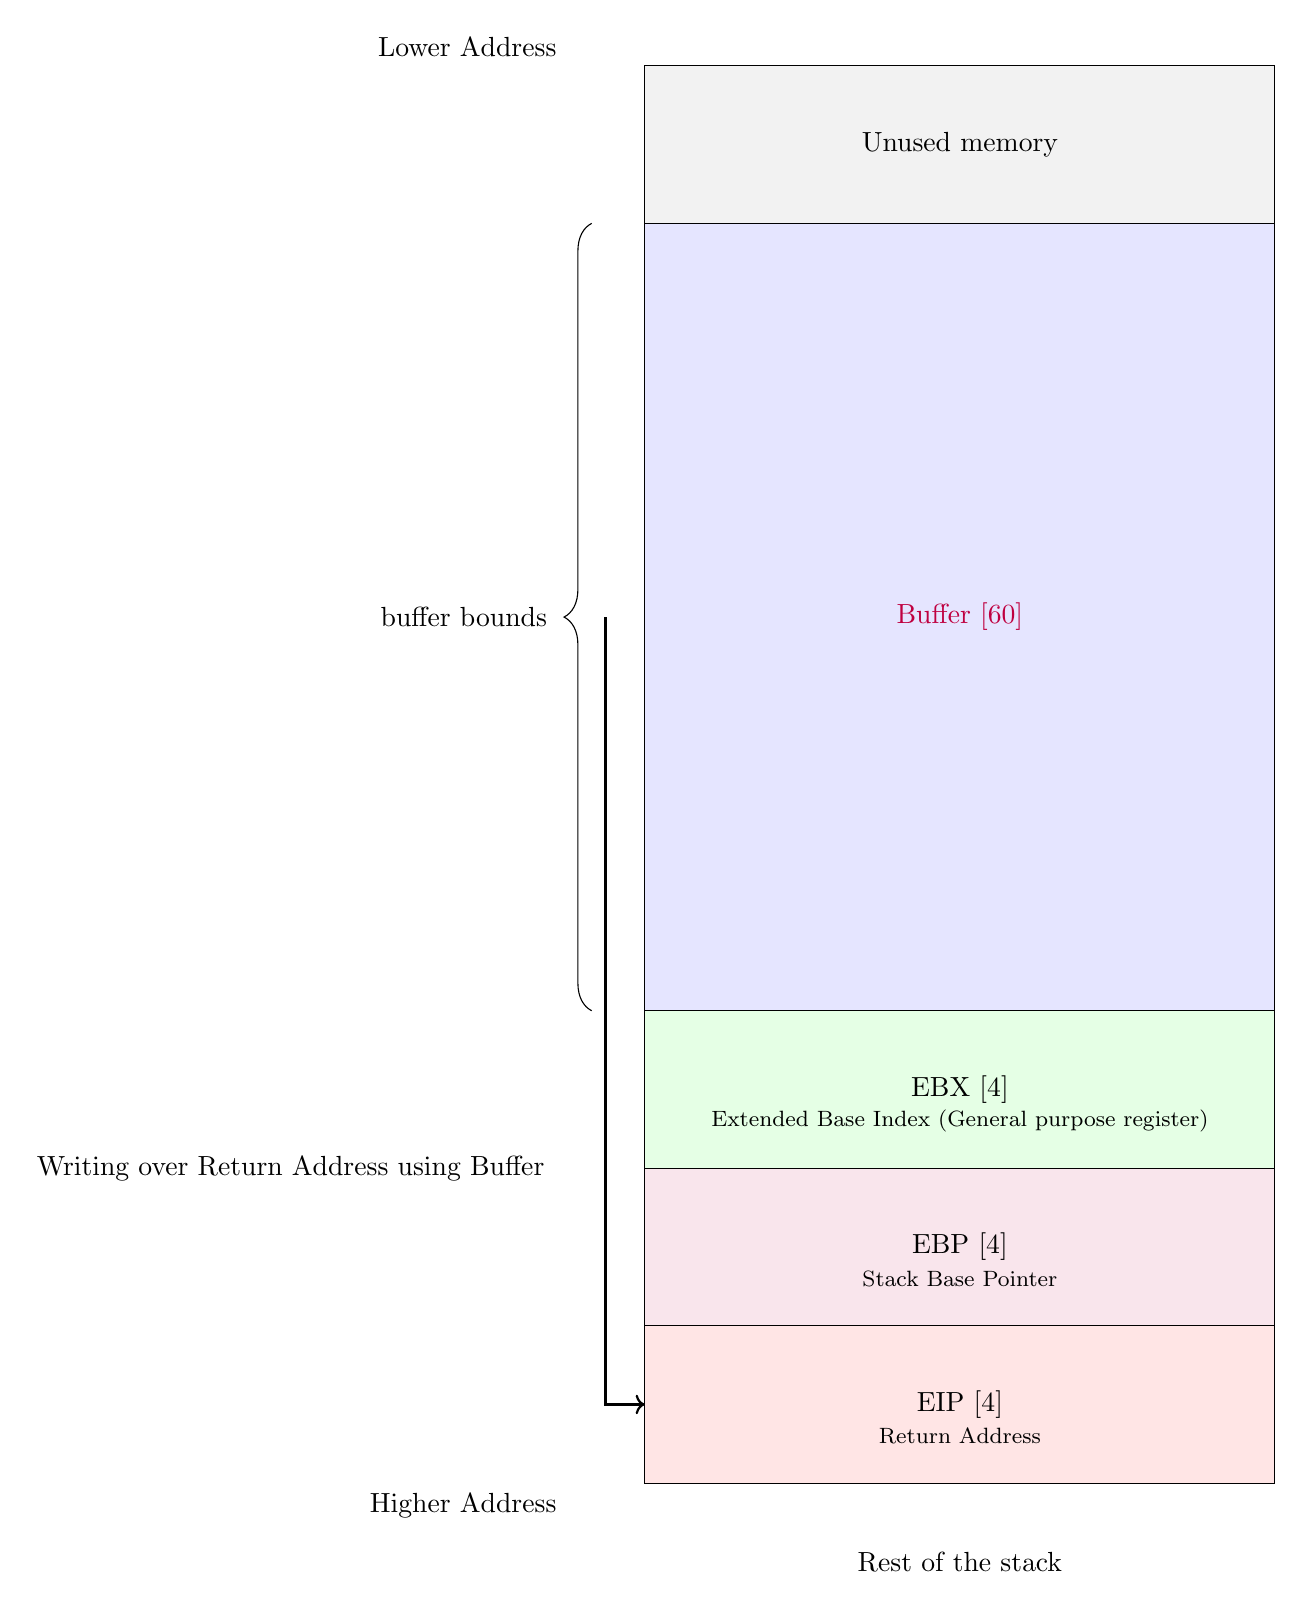
\begin{tikzpicture}

	% Dimensions
	\def\bufferheight{10}
	\def\boxheight{2}
	\def\boxwidth{8}
	
	% Unused memory
	\draw[fill=gray!10] (0, \bufferheight + 3*\boxheight) rectangle (\boxwidth, \bufferheight + 4*\boxheight);
	\node at (\boxwidth/2, \bufferheight + 3.5*\boxheight) {Unused memory};
	
	% Buffer
	\draw[fill=blue!10] (0, \boxheight*3) rectangle (\boxwidth, \bufferheight + 3*\boxheight);
	\node[text=purple] at (\boxwidth/2, \bufferheight/2 + 3*\boxheight) {Buffer [60]};
	
	% EBX
	\draw[fill=green!10] (0, 2*\boxheight) rectangle (\boxwidth, 3*\boxheight);
	\node at (\boxwidth/2, 2.5*\boxheight) {EBX [4]};
	\node at (\boxwidth/2, 2.3*\boxheight) {\footnotesize Extended Base Index (General purpose register)};
	
	% EBP
	\draw[fill=purple!10] (0, \boxheight) rectangle (\boxwidth, 2*\boxheight);
	\node at (\boxwidth/2, 1.5*\boxheight) {EBP [4]};
	\node at (\boxwidth/2, 1.3*\boxheight) {\footnotesize Stack Base Pointer};
	
	% EIP
	\draw[fill=red!10] (0, 0) rectangle (\boxwidth, \boxheight);
	\node at (\boxwidth/2, 0.5*\boxheight) {EIP [4]};
	\node at (\boxwidth/2, 0.3*\boxheight) {\footnotesize Return Address};
	
	% Rest of the stack
	\node at (\boxwidth/2, -0.5*\boxheight) {Rest of the stack};
	
	% Address labels
	\node[anchor=south east] at (-1, \bufferheight + 4*\boxheight) {Lower Address};
	\node[anchor=north east] at (-1, 0) {Higher Address};
	\draw[->, thick] (-0.5, \bufferheight/2 + 3*\boxheight) -- (-0.5,  0.5*\boxheight) -- (0,  0.5*\boxheight);
	\node at (-4.5, 2*\boxheight) {Writing over Return Address using Buffer};
	\draw [decorate,decoration={brace,amplitude=10pt,raise=5pt}] (-0.5, 3*\boxheight) -- (-0.5, 3*\boxheight+\bufferheight) node [black,midway,xshift=-1.8cm] {buffer bounds};

	\end{tikzpicture}
\end{center}	
The buffer overflow will overwrite the return address value such as the next instruction will be the one of the beginning of the buffer, containing the shellcode.

In order to do the exploit we use this command to launch the program:\\
	\begin{lstlisting}[breaklines=true]
		./main `perl -e ' print "\x31\xc0\x48\xbb\xd1\x9d\x96\x91\xd0\x8c\x97\xff\x48\xf7\xdb\x53\x54\x5f\x99\x52\x57\x54\x5e\xb0\x3b\x0f\x05AAAAAAAAAAAAAAAAAAAAAAAAAAAAAAAAAAAAAAAAAAAAA\xd0\xe0\xff\xff\xff\x7f";'`
	\end{lstlisting}
	\subsubsection{Debian Environment}
The end address must be replaced by the buffer address in little endian format.
The perl command is used to write binary number (such as address) as input to the program.
To compile the code, the options: "-fno-stack-protector" and "-z execstack" must be used because the canari detects the overflow and the non executable stack forbids code execution.
Also use the command setarch -RL bash to disable address randomization for the terminal you are using.
According to \href{https://www.securityweek.com/aslr-bypass-techniques-appearing-more-frequently-attacks/}{security week}, \href{https://www.bleepingcomputer.com/news/security/cisa-warns-of-samsung-aslr-bypass-flaw-exploited-in-attacks/}{bleeping computer} and \href{https://www.securityweek.com/aslr-bypass-techniques-appearing-more-frequently-attacks/}{another article from security week} it is possible to bypass ASLR.
According to \href{https://tc.gts3.org/cs6265/2020-spring/tut/tut04-ssp.html}{Information security lab} and \href{https://ctf101.org/binary-exploitation/stack-canaries/}{ctf101} and \href{https://ibm.github.io/system-security-research-updates/2021/06/18/spear-attacks-ssp-usecase}{ibm} it is possible to bypass the stack protector.
Canaries are critized as being not secure in \href{https://ar5iv.labs.arxiv.org/html/2003.05503}{Bypassing memory safety mechanisms through speculative control flow hijacks} research paper and ALSR is criticized in the same way in \href{https://www.researchgate.net/publication/346588673_Speculative_Probing_Hacking_Blind_in_the_Spectre_Era}{Speculative\_Probing\_Hacking\_Blind\_in\_the\_Spectre\_Era}.
The non executable stack forbids buffer overflow that aims at returning on the stack but more complex attacks will use the same idea (by calling a method in a library that contains a vulnerability, which with correct arguments, allows arbitrary code execution, or calling a method that is not supposed to be called at this point of the execution, causing chaos in the program) so to keep this example simple we will disable it.

\begin{tcolorbox}[colback=gray!5!white, colframe=gray!75!black, title=Output on classic \Gls{risc-v} environment (No CHERI protection)]
true return address: 0x555555555230\\
after strcpy\\
buf: 0x7fffffffe0d0\\
true return address: 0x7fffffffed0d0\\
\$ 
\end{tcolorbox}
The "\$" symbol demonstrate access to a shell. For example using "ls" command will print files in current directory.
\subsubsection{CHERI protected Arm Morello Environment}
On CHERI ARM \Gls{morello}, non executable stack is forbidden to execute. We will still try, because the fact the stack is non executable will not play a role in this program execution.
\begin{tcolorbox}[colback=gray!5!white, colframe=blue!75!black, title=Execution on CHERI environment]
true return address: 0x110a85\\
In-address space security exception (core dumped)
\end{tcolorbox}
The buffer overflow is prevented during strcpy. The writing occurs out of the bounds of the buffer pointer, so an error is thrown.
\subsection{Buffer Overflow On Integer cast to Pointer}
Buffer overflow can happen in internal structure. We saw previously that using a function pointer address failed because the pointer became invalid. But what about an integer that can be cast to a pointer ?

\lstinputlisting[numbers=none, caption=]{code/intStruct.c}
Use this command: perl -e 'print "aaa";' | ./test2 \\
In order to get the address a first time then do the overflow with the obtained address.
\subsubsection{RISC-V environment}

\begin{tcolorbox}[colback=gray!5!white, colframe=gray!75!black, title=Output on classic \Gls{risc-v} environment (No CHERI protection)]
f2:0x2109a4\\
0x2109a4\\
hacking
\end{tcolorbox}
\subsubsection{CHERI protected Arm Morello Environment}
Remember that CHERI bounds are not precise. The buffer size may not have expected size.
\begin{tcolorbox}[colback=gray!5!white, colframe=blue!75!black, title=Execution on CHERI environment]
f2:0x11094d\\
0x11094d\\
In-address space security exception
\end{tcolorbox}
Looking with \acrshort{gdb} we can see it is due to a Capability Tag fault which demonstrate that integer that can be cast into pointers are related to a capability tag.
\subsection{Buffer Overflow over Vulnerable function pointer pointer followed by object duplication using Offset to identify method pointer}

The main idea behind this attack is that if CHERI protects against out of bounds and usage in read or write of invalid pointers, it does not protect against out of bounds inside a structure and it allows invalid pointers to access their address value, which can be used to calculate an offset. If the offset is used without more control after an overflow modifying its value, it can allow an attacker to perturb the normal execution behavior of a program.
In order to illustrate this, I wrote the code of a vulnerable application that will be the target of an exploit, in which case the exploit theoretically allows an attacker to call any methods of an object, with some big assumptions about how the program is implemented and compiled: it requires a vulnerable structure with the possibility of a buffer overflow on a pointer on a function pointer inside the object, that can be called without control, the possibility of duplicating an object after a buffer overflow, and that the pointer on a function pointer value is calculated with an offset during the duplication. It also requires that the offset is calculated without further control of the result. 
CHERI protection can however easily mitigate this problem: using the option -Xclang -cheri-bounds=subobject-safe, the exploit can not happen. Any verification on either the offset value or the function call makes the exploit impossible to succeed.

In order to run the exploit, we need all the files from this \href{https://github.com/pglbgit2/exploit.git}{directory}, then follow README instructions. The code is also fully present in annex.
The simple application uses a structure with private information, a password and public information.
\lstinputlisting[numbers=none, firstline=15, lastline=27, caption= Structure]{code/exploit.c}

The objective of this exploit is to call the secret function which allows the attacker to change the password value inside the object, then print private information to prove the password was modified.
exploit.c goal is to simulate a very-basic multi user application (it stands for exploitable application). 
The functions are used to print and modify attributes. Here the most important is secret which is not supposed to be called directly by the user, which will modify the password of the structure, required to access private information. The function pointer pointer pptr is used to choose a function to call and then call it. When the function chose by the user does not exist, it doesn't change its value and then call the function it points.

% Dimensions
\def\boxheight{2}
\def\boxwidth{5}

\newcommand{\drawStruct}[4][]{
    % #1: Options de remplissage
    % #2: Coordonnée x de la structure
    % #3: Coordonnée y de la structure
    % #4: Liste des attributs

    \foreach \i [count=\j from 0] in {#4} {
        \draw[fill=green!10, #1] (#2, #3 - \j*\boxheight) rectangle 
        (#2 + \boxwidth, #3 - \j*\boxheight + \boxheight);
        \node at (#2 + \boxwidth/2, #3 - \j*\boxheight + 0.5*\boxheight) {\i};
    }
}
First we initialize a structure, supposing normal usage of application.
\begin{center}
\begin{tikzpicture}[scale = 0.75]
	\node at (\boxwidth/2, 3) {Initial State};
	\drawStruct{0}{0}{ password, privateInformation, buffer, publicInformation, pptr, f1ptr, f2ptr, f3ptr, f4ptr, secret}
\end{tikzpicture}
\end{center}
Then we suppose the attacker has control over the input. The application is supposed to keep private information private to those who know the correct password. However, the attacker will use an exploit that will allow him to print it without ever knowing the password.
He will first do a buffer overflow using the buffer that receive user input, allowing him to change the pptr value. However this leads to the invalidation of the pointer, meaning its not possible to dereference it.
\begin{center}
\begin{tikzpicture}[scale = 0.75]
	\node[align=center] at (\boxwidth/2, 3) {Doing buffer overflow from buffer on pointer of function pointer (pptr)\\making it points to pointer to secret function};
	\drawStruct{0}{0}{ password, privateInformation, buffer, publicInformation, pptr, f1ptr, f2ptr, f3ptr, f4ptr, secret}
	\node[color=red] at (-2.2, -\boxheight*5/2) {Buffer Overflow};
	\draw[->, line width=2pt, color=red] (-0.3, -\boxheight*3/2) -- (-0.3, -\boxheight*7/2);
	\draw[->, thick, color=red] (0, -\boxheight*7/2) -- (-1, -\boxheight*7/2)-- (-1, -\boxheight*17/2)-- (0, -\boxheight*17/2);
	\node[color=red] at (\boxwidth/2, -\boxheight*11/3) {(invalid)};
	
\end{tikzpicture}
\end{center}
The attacker knows he can not dereference pptr because it will lead to a security exception throw. However he can duplicate a structure.
During the duplication, an offset is used to get the pointer to the function pointer. This is one example of an offset usage that can be used in a malicious case. In this case, as it is allowed, the pptr of the duplicated object is still valid.
That means its possible to call the secret function from the duplicated object directly even if it was not supposed to happen in the original code.
\lstinputlisting[numbers=none, firstline=100, lastline=118, caption=Duplication]{code/exploit.c}

\begin{center}
\begin{tikzpicture}[scale = 0.75]
	\node[align=center] at (\boxwidth/2+5, 3) {Duplicating the object \\ Using offset to determine pptr value};

    \drawStruct{0}{0}{ password, privateInformation, buffer, publicInformation, pptr, f1ptr, f2ptr, f3ptr, f4ptr, secret}
    \drawStruct{8}{0}{ password, privateInformation, buffer, publicInformation, pptr, f1ptr, f2ptr, f3ptr, f4ptr, secret}
	\draw[-, thick] (\boxwidth, -\boxheight*7/2) -- (\boxwidth+1, -\boxheight*7/2) -- (\boxwidth+1, -\boxheight*17/2) -- (\boxwidth, -\boxheight*17/2);
	\draw[-, thick] (\boxwidth+1, -\boxheight*12/2) -- (\boxwidth+2, -\boxheight*12/2)-- (\boxwidth+2, -\boxheight*7/2)-- (\boxwidth+3, -\boxheight*7/2);
	\draw[->, thick] (8+\boxwidth, -\boxheight*7/2) -- (9+\boxwidth, -\boxheight*7/2)-- (9+\boxwidth, -\boxheight*17/2)-- (8+\boxwidth, -\boxheight*17/2);
	\node at (8+\boxwidth/2, -\boxheight*11/3) {(valid)};
	\node[color=red] at (\boxwidth/2, -\boxheight*11/3) {(invalid)};
	\filldraw[fill=white] (\boxwidth+1,-\boxheight*12/2) circle [radius=0.5];
	\node at (\boxwidth+1,-\boxheight*12/2) {$-$};
	\draw[->, thick, color=red] (0, -\boxheight*7/2) -- (-1, -\boxheight*7/2)-- (-1, -\boxheight*17/2)-- (0, -\boxheight*17/2);
\end{tikzpicture}
\end{center}
The secret function allows the attacker to change the password, and thus, printing private information and having full control over the structure he duplicated.

To conclude, this is one example of a usage of how a buffer overflow followed by the use of an offset can be problematic.
However, this example is still very unrealistic. C code isn't usually write like this and C++ class don't have attributes that are function pointer leading to their methods: they have a virtual method table that all instance of a class can access using a single pointer which is before all attributes. Meaning it would be impossible under CHERI protection to modify a method pointer. This could still be problematic if using a pointer to pointer as an attribute and calculating an offset with it, but it would be not probable that the exploit of such a vulnerability leads to arbitrary method call, as in this case.
There are still two subtleties: even if a vulnerability exploit will fail, attackers can provoke faults at will, meaning handling of those faults have to be considered. If the usage of an offset between two pointer, one that could be overflowed, the application could encounter problems that are not handled, leading to DOS (Denial Of Service).


\section{Cyberphys Demonstration}
\subsection{Demonstration context}
This application is positioned in an  context using a CAN data bus. The application represent the ECU and controls user's input (brakes, steering wheel) and must react accordingly. The data is transmitted via a CAN bus.
The application is coded entirely in C.
It is assumed that an attacker has access to this data bus. The attack scenario under consideration poses problems of availability, integrity and confidentiality because the J1939 protocol used in this application is vulnerable to a buffer overflow attack, enabling the attacker, after successful exploitation of the vulnerability, to take total control of the vehicle. The demonstration shows that on a conventional system, the system is compromised, but on a system benefiting from CHERI protection, a security exception is lifted. \\
The application runs in two environments: a FreeRTOS system on RISC-V architecture and a CHERI-FreeRTOS system on CHERI-RISC-V architecture. The application is called Cyberphys.
\begin{figure}
        \begin{center}
                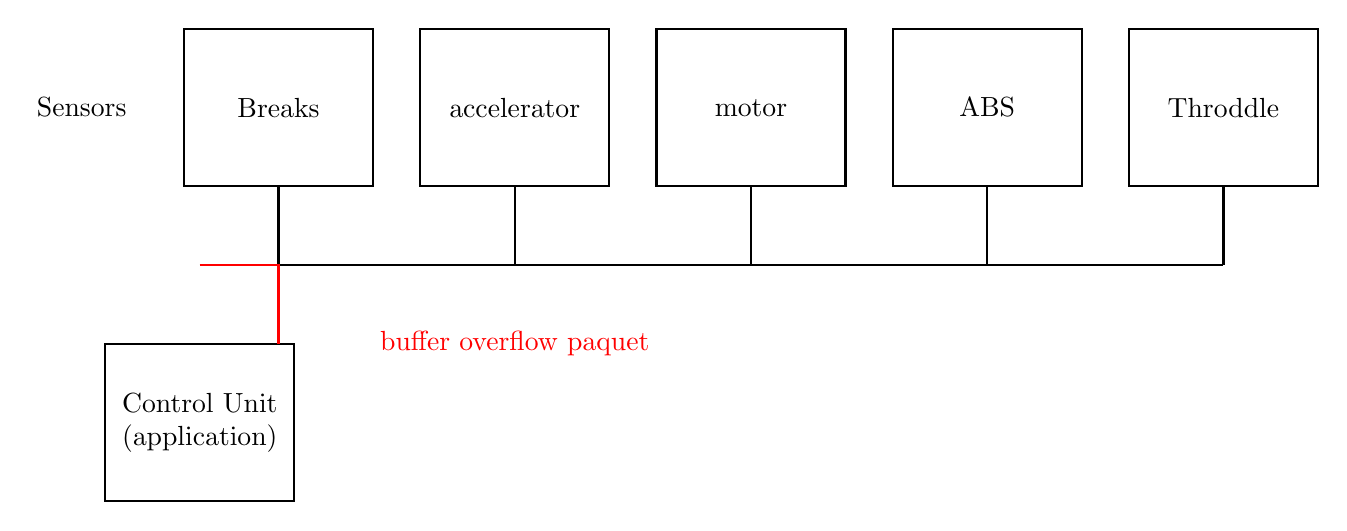
\begin{tikzpicture}

                % Draw the CAN bus line
                \draw[thick] (0, 0) -- (13, 0);
                
                % Draw the components (rectangles) connected to the bus
                \foreach \x in {1, 4, 7, 10, 13} {
                    \draw[thick] (\x, 0) -- (\x, 1); % Connect component to bus
                    \draw[thick] (\x-1.2, 1) rectangle (\x+1.2, 3); % Draw component
                }
                \draw[thick] (1, 0) -- (1, -1); % Connect component to bus
                \draw[thick] (-1.2, -1) rectangle (1.2, -3); % Draw component

                % Add labels to components
                \node at (1, 2) {Breaks};
                \node at (4, 2) {accelerator};
                \node at (7, 2) {motor};
                \node at (10, 2) {ABS};
                \node at (13, 2) {Throddle};
                \node at (-1.5, 2) {Sensors};
                \node[align=center] at (0, -2) {Control Unit \\ (application)};
                \draw[thick, red] (0, 0) -- (1, 0) -- (1, -1);
                \node[red] at (4,-1) {buffer overflow paquet};

                \end{tikzpicture}
        \end{center}
        \caption{Bus CAN} 
		\label{fig:canbus}

\end{figure}

\subsection{Demonstration Theory}
A remark by Dr. Hesham Almatory in his thesis \cite{almatary2022compartos} is that the raising of an exception effectively prevents the exploitation of a vulnerability aimed at a subtle objective such as the execution of arbitrary code, but does not prevent the \Gls{dos}.
In other words, the system is not corrupted (the integrity and confidentiality of the system are preserved) when a security exception is raised, but stopped (availability is non-existent). Losing control of a vehicle can be problematic for a number of obvious reasons. Dr Hesham Almatory's first solution, which he describes as naive, is to restart the entire system. According to his experiments, this takes approximately two seconds. That may not sound like much, but in an emergency braking situation it can be problematic. This could be a scenario involving multiples attacks: the attacker can carry out his attack in a loop and force an immediate reboot as soon as the system becomes functional again. 
The second solution proposed by Dr Hesham consists of compartmentalising the application using a method of his own invention called CompartOS, which is based on CHERI capabilities and is carried out automatically during the linking stage carried out by the compiler. Four solutions are proposed: restarting the offending compartment (requires minimal implementation effort, but is not always possible, it requires to be able to create snapshots of a compartment and restore it), modifying the code to include error handling (requires a small implementation effort but requires knowledge of the errors that can be handled), using a handler function (that requires knowing what the problematic elements are, to free them and realocate them) or 'killing' the compartment (this solution is only possible in cases where the compartment is not crucial, such as a music player). Depending on the type of problem, each of the four solutions may be necessary. In this case, the handling function is called.
To catch security exception thrown by the hardware, Dr Hesham had to modify the CHERI-FreeRTOS kernel : when a architectural exception is thrown it is catched by the OS, who print the fault but more importantly forward the fault to a software handler which is in this case the compartment handler identified by its name (CheriFreeRTOS\_FaultHandler), and if not found, uses return error, compartment kill or micro reboot depending on the option given to compartmentalize (by default it is return error).

By using simple function handling, consisting of allocating again the corrupted buffer in another memory area, the compartment returns to a functional state in thirty micro-seconds, however, the previous allocated memory is not released and this can lead to a exhaustion of memory resources in the long term. With a little implementation effort, it is possible to specify the release of allocated memory and thus avoid the backlog. This takes sixty microseconds. In this way, system availability is maintained and the effectiveness of CompartOS based on CHERI protections is demonstrated.
The application used in the demonstration is not complete (it does not simulate all the components of a vehicle): it is a simplified version comprising only the management of data from the CAN bus, using the J1939 protocol, as well as a task updating the information received from the sensors (non-existent in this case). The aim is simply to demonstrate the presence and possible exploitation of a buffer overflow without the CHERI protection.

\newcommand{\drawstack}[3]{
        \draw (#1,#2) rectangle (#1+4,#2+#3);   
        \foreach \v in {1, ..., #3}{
                \draw[-] (#1,\v+#2) -- (#1+4,#2+\v);
        }
}
\newcommand{\drawdemostack}[2]{
        \drawstack{#1}{#2}{4};
        \drawstack{#1}{#2+5}{3};

        \node at (#1+2,#2+0.5) {...};
        \node at (2+#1,#2+7.5) {...};
        \node at (2+#1,6.5+#2) {global buffer};
        \node at (2+#1,1.5+#2) {vulnerable buffer};
        \node at (2+#1,#2+5.5) {...};
}
\begin{figure}
        \begin{center}
                \begin{tikzpicture}[scale=0.75]
                       \drawdemostack{0}{0}
                        \draw [decorate,decoration={brace,amplitude=10pt,raise=5pt}] (0, 5) -- (0, 8) node [black,midway,xshift=-2.5cm] {Global Variable};
                        \draw [decorate,decoration={brace,amplitude=10pt,raise=5pt}] (0, 1) -- (0, 4) node [black,midway,xshift=-2.5cm] {Tasks memory};
                        \draw [decorate,decoration={brace,amplitude=10pt,raise=5pt}] (0, 0) -- (0, 1) node [black,midway,xshift=-2.4cm] {Unused Memory};
                        \draw [decorate,decoration={brace,amplitude=10pt,raise=5pt}] (4, 2) -- (4, 1) node [black,midway,xshift=3.2cm] {Protocol J1939 variables};
                \end{tikzpicture}
        \end{center}
        \caption{Demonstration: Initial State} 
		\label{fig:demo_init}

\end{figure}
In the initial state, \ref{fig:demo_init} and throughout execution, the program's memory space is divided into three parts: the tasks, the global variables and the variables used in the functions called by the tasks.

\begin{figure}
        \begin{center}
                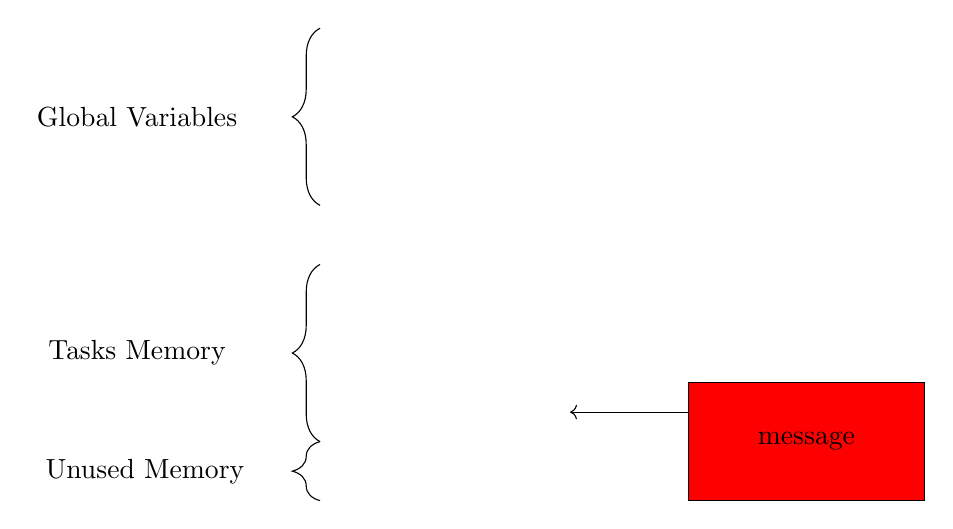
\begin{tikzpicture}[scale=0.75]
                        \fill [red] (6,0) rectangle (10,2);
                        \draw[->] (6,1.5) -- (4,1.5);
                        \draw[black] (6,0) rectangle (10,2);   
                        \drawdemostack{0}{0}
                        \node at (8,1) {message};
                        \draw [decorate,decoration={brace,amplitude=10pt,raise=5pt}] (0, 5) -- (0, 8) node [black,midway,xshift=-2.5cm] {Global Variables};
                        \draw [decorate,decoration={brace,amplitude=10pt,raise=5pt}] (0, 1) -- (0, 4) node [black,midway,xshift=-2.5cm] {Tasks Memory};
                        \draw [decorate,decoration={brace,amplitude=10pt,raise=5pt}] (0, 0) -- (0, 1) node [black,midway,xshift=-2.4cm] {Unused Memory};
                \end{tikzpicture}
        \end{center}
        \caption{Demonstration: Message Reception} 
		\label{fig:demo_paquet}

\end{figure}
When the \ref{fig:demo_paquet} message is received, it is reconstituted from the multiple packets requiring a certain format sent in the CAN BUS. 

\begin{figure}
        \begin{center}
                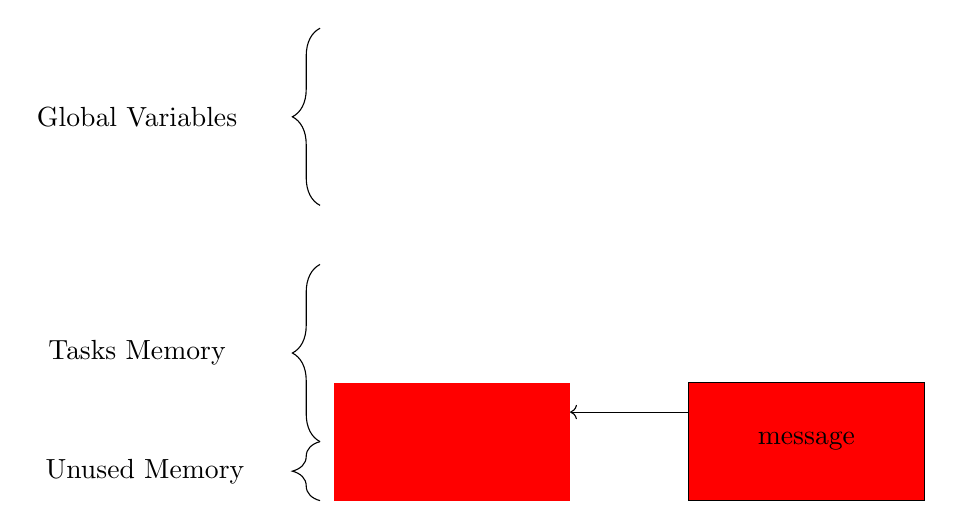
\begin{tikzpicture}[scale=0.75]
                        \fill [red] (6,0) rectangle (10,2);
                        \draw[->] (6,1.5) -- (4,1.5);
                        \node at (8,1) {message};
                        \draw[black] (6,0) rectangle (10,2);   
                        \fill [red] (0,0) rectangle (4,2);
                        \drawdemostack{0}{0}
                        \draw [decorate,decoration={brace,amplitude=10pt,raise=5pt}] (0, 5) -- (0, 8) node [black,midway,xshift=-2.5cm] {Global Variables};
                        \draw [decorate,decoration={brace,amplitude=10pt,raise=5pt}] (0, 1) -- (0, 4) node [black,midway,xshift=-2.5cm] {Tasks Memory};
                        \draw [decorate,decoration={brace,amplitude=10pt,raise=5pt}] (0, 0) -- (0, 1) node [black,midway,xshift=-2.4cm] {Unused Memory};
                \end{tikzpicture}
        \end{center}
        \caption{Demonstration: First Buffer Overflow} 
		\label{fig:demo_overflow}

	\end{figure}

The first buffer overflow \ref{fig:demo_overflow} occurs when the buffer in which the function implementing the J1939 protocol copies the entire received message without checking its size. On a conventional FreeRTOS system, the buffer overflow goes unnoticed.
On a CHERI-FreeRTOS system, the buffer overflow attempt will raise a security exception due to the buffer being bound. On a compartmentalised system, the error handling will call a handler which will free the memory used by the protocol and instantiate it again.
\begin{figure}
        \begin{center}
                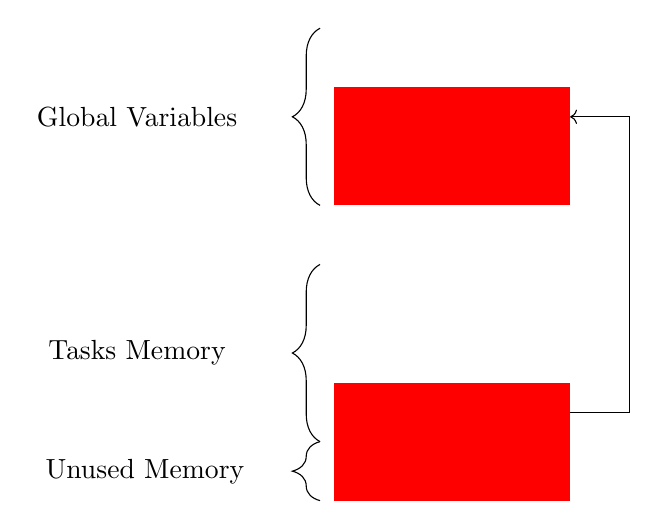
\begin{tikzpicture}[scale=0.75]
                        \draw[->] (4,1.5) -- (5,1.5) -- (5,6.5) -- (5,6.5) -- (4,6.5);
                        \fill [red] (0,0) rectangle (4,2);
                        \fill [red] (0,7) rectangle (4,5);

                        \drawdemostack{0}{0}
                        \draw [decorate,decoration={brace,amplitude=10pt,raise=5pt}] (0, 5) -- (0, 8) node [black,midway,xshift=-2.5cm] {Global Variables};
                        \draw [decorate,decoration={brace,amplitude=10pt,raise=5pt}] (0, 1) -- (0, 4) node [black,midway,xshift=-2.5cm] {Tasks Memory};
                        \draw [decorate,decoration={brace,amplitude=10pt,raise=5pt}] (0, 0) -- (0, 1) node [black,midway,xshift=-2.4cm] {Unused Memory};
                \end{tikzpicture}
        \end{center}
        \caption{Demonstration: Copy and second Buffer Overflow} 
		\label{fig:demo_copy}

\end{figure}
The next step, when the buffer is copied to a global variable in an uncontrolled way \ref{fig:demo_copy}, where the exploitation of the vulnerability makes sense, therefore does not occur on a CHERI-FreeRTOS system. On the other hand, on a FreeRTOS system, the buffer will overflow onto global variables and replace their values. In this version of this demonstration, this simply stops the execution of the program by replacing used variables that are supposed to have certain values, causing a fault when used. In the original demonstration, the application included an authentication key, vulnerable to a buffer overflow on the global buffer, which was used to accept instructions during over-the-air updates, giving the attacker total control of the vehicle. 
\newcommand{\threeRect}[5]{
        \draw (#1,#2) rectangle (#1+5,#2+1);
        \draw (#1,#2+1) rectangle (#1+5,#2+2);
        \draw (#1,#2+2) rectangle (#1+5,#2+3);
        \node at (#1+2.5,0.5) {#3};
        \node at (#1+2.5,1.5) {#4};
        \node at (#1+2.5,2.5) {#5};
}
\begin{figure}
        \begin{center}
                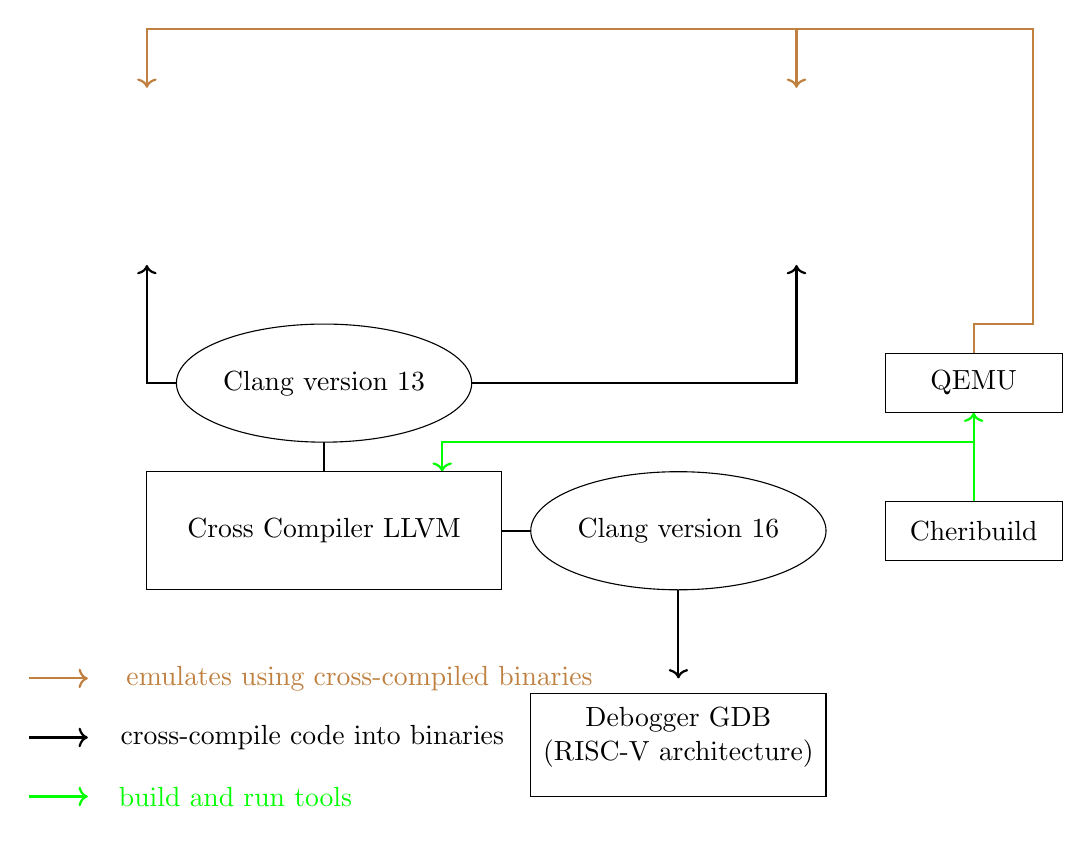
\begin{tikzpicture}[scale=0.75]
                        \threeRect{6}{0}{\Gls{cheri-risc-v}}{\Gls{cheri-freertos}}{Cyberphys};
                        \threeRect{-6}{0}{\Gls{risc-v}}{\Gls{freertos}}{Cyberphys};
                        \threeRect{0}{0}{Architecture}{\acrshort{os}}{Application};
                        \draw[->, thick] (0, -3.5) -- (0, -2)-- (-3, -2) --(-3, 0);
                        \draw[->, thick] (0, -2)-- (8, -2) --(8, 0);
                        \draw[->, thick, brown] (11, -1.5) -- (11, -1) -- (12, -1) -- (12, 4)-- (8, 4)-- (8, 3);
                        \draw[->, thick, brown] (8, 4) --(-3, 4)--(-3, 3);
                        \draw[->, thick, brown] (-5, -7) --(-4, -7);
                        \draw[->, thick] (-5, -8) --(-4, -8);

                        \filldraw[fill=white] (0,-2) ellipse (2.5cm and 1 cm);
                        \draw[->, thick] (3, -4.5)-- (6, -4.5) --(6, -7);

                        \filldraw[fill=white] (6,-4.5) ellipse (2.5cm and 1 cm);

                        \node at (6,-4.5) {Clang version 16};
                        \node at (11,-4.5) {Cheribuild};
                        \draw[->, thick, green] (11, -4) -- (11, -2.5);
                        \draw[->, thick, green] (11, -3) -- (2, -3) -- (2, -3.5);
                        \draw[->, thick, green] (-5, -9) -- (-4, -9);

                        \node at (0,-2) {Clang version 13};
                        \node[align=center] at (6,-8) {Debogger GDB\\ (RISC-V architecture)};
                		\draw (3.5,-9) rectangle (8.5,-7.25);

                        \node at (11,-2) {QEMU};
                        \node[brown] at (0.6,-7) {emulates using cross-compiled binaries};
                        \node[green] at (-1.5,-9) {build and run tools};

                        \node at (-0.2,-8) {cross-compile code into binaries};

                        \node[align=center] at (0,-4.5) {Cross Compiler LLVM};
                        \draw (-3,-5.5) rectangle (3,-3.5);
                        \draw (9.5,-5) rectangle (12.5,-4);
                        \draw (9.5,-2.5) rectangle (12.5,-1.5);
                        %\twoGear{0}{-4}
                \end{tikzpicture}
        \end{center}
        \caption{Demonstration Build} 
		\label{fig:cyberphys}
\end{figure}
The demonstration is build using \href{https://github.com/CTSRD-CHERI/cheribuild}{cheribuild} tool, to build LLVM (a cross compiler) and QEMU (an emulator). LLVM is then used to cross compile the various OS on top of the desired architecture: here FreeRTOS on top of RISC-V and CHERI-FreeRTOS on top of CHERI-RISC-V.


\subsection{Demonstration Reproduction}
The demonstration's application code is in FreeRTOS/Demo/RISC-V-Generic/demo/cyberphys and FreeRTOS/Demo/RISC-V\_Galois\_demo/cyberphys repository.
\lstinputlisting[numbers=none, caption=,language=bash, lastline=90]{code/CHERI_FREERTOS_DEMO.sh}

Its possible to modify the attack code in many ways: augmenting the size of the buffer and the send length, sending multiple message in a loop (requiring a minimum delay to avoid DOS on your own computer, and avoid sending too many paquets at the same time, because they will cause the emulation to crash).
To exit QEMU, use: Ctrl+a+x.
When running the attack code on a FreeRTOS environment, the expected output is that the message will be received with (recv\_can\_message) prints, then the program will stop. Its possible to add additional prints to have more information. The code to modify is on ~/cheri/freertos/FreeRTOS/Demo/Risc-V-Generic/demo/cyberphys/ .
On a CHERI-FreeRTOS environment, if using debug mode, a security exception will be printed, otherwise the same result as from the FreeRTOS environment will be observed.
On a compartmentalized CHERI-FreeRTOS environment, a security exception will be printed \ref{sec:cyberphys-error}, and the program will continue running after handling the error using the handling function in j1939.c file. It will, as explained in the theory section, free the corrupted buffer and allocate it again.
\begin{figure}[h!]
	\includegraphics[scale=0.4]{images/SecurityException.png}
	\caption{Security Exception under Compartmentalised Cheri-FreeRTOS Execution}
	\label{sec:cyberphys-error}
\end{figure}

The fact the program resume after handling a fault is a proof that the availability of the system is maintained. The fault is a proof that the integrity and confidentiality of the system are maintained.
\clearpage 
\bibliographystyle{plain}
\bibliography{source}
\addcontentsline{toc}{section}{References}

\clearpage 
\appendix
\section{Annex 1: Exploit Code}
This code can also be found \href{https://github.com/pglbgit2/exploit.git}{here}
\lstinputlisting[numbers=none, caption=exploit.c]{code/exploit.c}

\lstset{ % Define settings for the listings package
    language=Python, % Set the language to Python
    basicstyle=\ttfamily, % Use typewriter font
    keywordstyle=\color{blue}, % Set keywords to blue
    stringstyle=\color{red}, % Set strings to red
    commentstyle=\color{darkgreen}, % Set comments to green
    breaklines=true, % Enable line breaks
    showstringspaces=false, % Don't show spaces in strings
    tabsize=4 % Set tab size to 4 spaces
}
We use a python script to manage binary input easily (it is possible to do without, it is just more complex for the user). 
BOF.py goal is to facilitate the input management (binary writing) and address retrieving automatically.
\lstinputlisting[numbers=none, caption=BOF.py]{code/BOF.py}
fileMerger.py goal is to merge files.
\lstinputlisting[numbers=none,caption=FileMerger.py]{code/fileMerger.py}
InputExec.py goal is to launch exploit program and return its output.
\lstinputlisting[numbers=none, caption=InputExec.py]{code/InputExec.py}


Here is an example of begin.txt file: its goal is to print the target function address so that BOF.py can write the inject file.
\begin{center}
\begin{tcolorbox}[colback=white!5!white, colframe=gray!75!black, title=begin.txt]
create\\
qwerty\\
call\\
f4\\
qwerty\\
something\\
something\\
call\\
f3\\
qwerty\\
debug\\
exit\\
f3
\end{tcolorbox}

Here is an example of init file: its goal is to initialize some non malicious user data
\begin{tcolorbox}[colback=white!5!white, colframe=gray!75!black, title=init]
create\\
apassword\\
call\\
f4\\
apassword\\
a private information\\
a public information\\
call\\
f3
\end{tcolorbox}
Here is an example of end.txt: its goal is to be malicious input that will retrieve the data by performing the end of the exploit.
\begin{tcolorbox}[colback=white!5!white, colframe=gray!75!black, title=end.txt]
duplicate\\
move\\
1\\
debug\\
call\\
t\\
Y\\
aaaa\\
call\\
f3\\
aaaa\\
exit\\
\end{tcolorbox}
\end{center}
\end{document}
